\section{Inducción y Recurrencia}
\subsection{Introducción a los naturales}
En el estudio de los números naturales es necesario establecer un punto de partida y a partir de ahí, podremos definir operaciones básicas como la suma, el producto o el orden. Para ello, usaremos de punto de partida los axiomas de Peano y de esta forma llegaremos a todo lo que conocemos sobre los números naturales.
\subsection{Axiomática de Peano}
Supongamos que existe un conjunto $\mathbb{N}$. Los elementos de este conjunto se llaman números naturales.
\begin{ndef}[Axiomas de Peano]
    Los axiomas que definen a $\nat$ son los siguientes:
    \begin{enumerate}[label=\emph{A\arabic*}]
        \item\label{a0} El cero es un número natural. $0 \in \mathbb{N}$
        \item\label{a1} El siguiente de un número natural es un número natural. Si $n \in \mathbb{N} \Rightarrow \sigma(n) \in \mathbb{N}$
        \item\label{a2} Cero no es el siguiente de ningún número natural. $\forall n \in \mathbb{N}$, $\sigma(n) \neq 0$
        \item\label{a3} Si los siguientes de dos números naturales son iguales, entonces los números naturales son iguales. $\forall m,n \in \mathbb{N}, \sigma(n) = \sigma(m) \Rightarrow m = n$
        \item\label{a4} Si un subconjunto de números naturales tiene el cero y siempre que tiene un número tiene a su siguiente, entonces el subconjunto son todos los números naturales.
    \end{enumerate}
\end{ndef}

\begin{nota}
    Podemos definir $\sigma(n) = n + 1$ $\forall n \in \nat$.
\end{nota}

\begin{nth}
    Todo número natural es distinto del siguiente. $\forall n \in \nat n \neq \sigma(n)$
\end{nth}
\begin{proof}
    Sea $A = \{x \in \nat : x \neq \sigma(x)\}$: \\
    Como $0 \neq \sigma(0)$, resulta $0 \in A$.
    Supongamos ahora $n \in A$, es decir, $n \neq \sigma(n)$, luego $\sigma(n) \neq \sigma(\sigma(n))$, por tanto, $\sigma(n) \in A$.
    Luego $A = \nat$.
\end{proof}

\begin{nth}
    Para cada número natural distinto de cero, existe un único número natural del que es su siguiente. $\forall n \in \nat (n \neq 0 \Rightarrow \exists! m \in \nat$ tal que $x = \sigma(m))$
\end{nth}
\begin{proof}
    Sea $A = \{x \in \nat : x = 0$ o $m \in \nat$ tal que $x = \sigma(m)\}$:\\
    Como $0 = 0$, resulta $0 \in A$. Supongamos ahora $n \in A$, es decir, $n = 0$ o $n = \sigma(m)$. En cualquier caso, $\sigma(n) = \sigma(n)$, por tanto $\sigma(n) \in A$. Luego $A = \nat$. \\
    La unicidad es consecuencia de $A4$.
\end{proof}

\subsection{Aritmética natural}
\subsubsection{Suma de naturales}
\begin{nth}
    Existe una única $+ : \nat \times \nat \rightarrow \nat$ tal que $\forall m,n \in \nat$ verifica:
    \begin{itemize}
        \item $m + 0 = m$
        \item $m + \sigma(n) = \sigma(m + n)$
    \end{itemize}
\end{nth}
\begin{properties}
    Para todo $m,n,p \in \nat$ se cumple:
    \begin{enumerate}
        \item Todo número natural es 0 o es el siguiente de un número natural.
        \item $m + 0 = 0 + m = m$.
        \item $m + 1 = 1 + m = \sigma(m)$.
        \item $(m + n) + p = m + (n + p)$.
        \item $m + n = n + m$.
        \item Si $m + p = n + p$, entonces $m = n$.
        \item Si $m + n = 0$, entonces $m = n = 0$.
    \end{enumerate}
\end{properties}

\subsubsection{Producto de naturales}
\begin{nth}
    Existe una única $\cdot : \nat \times \nat \rightarrow \nat$ tal que $\forall m,n \in \nat$ verifica:
    \begin{itemize}
        \item $m \cdot 0 = 0$
        \item $m \cdot \sigma(n) =  m \cdot n + m$
    \end{itemize}
\end{nth}

\begin{properties}
    Para todo $m,n,p \in \nat$ se cumple:
    \begin{enumerate}
        \item $0 \cdot m = m \cdot 0 = 0$.
        \item $1 \cdot m = m \cdot 1 = m$.
        \item $(m + n) \cdot p = m \cdot p + n \cdot p$.
        \item $m \cdot n = n \cdot m$.
        \item Si $(m \cdot n) \cdot p = m \cdot (n \cdot p)$.
        \item Si $m \cdot n = 0$, entonces $m = 0$ o $n = 0$.
    \end{enumerate}
\end{properties}

\subsubsection{Potencias de naturales}
\begin{nth}
    Existe una única $\square^{\square} : \nat \times \nat \rightarrow \nat$ tal que $\forall m,n \in \nat$ verifica:
    \begin{itemize}
        \item $m^{0} = 1$
        \item $m^{\sigma(n)} =  m^{n} \cdot m$
    \end{itemize}
\end{nth}

\begin{properties}
    Para todo $m,n,p \in \nat$ se cumple:
    \begin{enumerate}
        \item $0^{0} = 1$.
        \item $0^{n} = 0$ para $1 \leq n$.
        \item $1^{n} = 1$.
        \item $m^{n+p} = m^{n} \cdot m^{p}$.
        \item Si $m^{n \cdot p} = (m^{n})^{p}$.
    \end{enumerate}
\end{properties}

\subsubsection{El orden de los naturales}
Primero definamos en qué consiste una relación de orden:
\begin{ndef}
    Sea $(A,R)$ un par ordenado con $A$ un conjunto no vacío y $R$ una relación binaria definida en $A$, entonces se dice que $R$ es una \textbf{relación de orden} si es:
    \begin{itemize}
        \item \textbf{Reflexiva}: Todo elemento de $A$ está relacionado consigo mismo. Es decir, $\forall x\in A,\ xRx$.
        \item \textbf{Antisimétrica}: Si dos elementos de $A$ se relacionan entre sí, entonces ellos son iguales. Es decir, $\forall x,y\in A,\ xRy,\ yRx \ \Rightarrow \ x=y$.
        \item \textbf{Transitiva}: Si un elemento de $A$ está relacionado con otro, y ese otro a su vez se relaciona con un tercero, entonces el primero estará relacionado también con este último. Es decir, $\forall x,y,z\in A,\;xRy,yRz\Rightarrow xRz$.
    \end{itemize}
\end{ndef}
\begin{ndef}[Orden]
    Dados $m,n \in \nat$ definimos m es menor o igual que n $(m \leq n)$ si $\exists x \in \nat$ tal que $m + x = n$. Lo podemos representar como $(\nat,\leq)$.
\end{ndef}

\begin{properties}
    Para todo $m,n,p \in \nat$ se cumple:
    \begin{enumerate}
        \item $m \leq m$.
        \item Si $m \leq n$ y $n \leq m$, entonces $m = n$.
        \item Si $m \leq n$ y $n \leq p$, entonces $m \leq p$.
        \item $m \leq n$ o $n \leq m$.
        \item Si $m \leq n$, entonces $\exists! p \in \nat$ tal que $m + p = n$ y lo llamamos n menos m $(n - m)$.
        \item Si $m \leq n$, entonces $m + p \leq n + p$.
        \item Si $m \leq n$, entonces $m \cdot p \leq n \cdot p$.
        \item Si $m \cdot p \leq n \cdot p$ y $p \neq 0$, entonces $m \leq n$.
        \item Si $m \cdot p = n \cdot p$ y $p \neq 0$, entonces $m = n$.
    \end{enumerate}
\end{properties}

\subsubsection{Divisibilidad en $\nat$}
\begin{ndef}[Divisibilidad]
    Dados $m,n \in \nat$ definimimos m divide a n $(m|n)$ si $\exists x \in \nat$ tal que $m \cdot x = n$.
\end{ndef}

\begin{properties}
    Para todo $m,n,p \in \nat$ se cumple:
    \begin{enumerate}
        \item $m|m$.
        \item Si $m|n$ y $n|m$, entonces $m = n$.
        \item Si $m|n$ y $n|p$, entonces $m|p$.
        \item Si $m|n$, entonces $\exists! p \in \nat$ tal que $m \cdot p = n$ y lo llamamos n partido por m $\left( \frac{n}{m} \right)$.
    \end{enumerate}
\end{properties}

\subsection{Principio de inducción}
\begin{nth}
    Las tres propiedades que siguen son equivalentes:
    \begin{enumerate}
        \item \textbf{Principio de inducción}. Si $A \subseteq \nat$ cumple $0 \in A$ y $(n \in A \Rightarrow n + 1 \in A)$, entonces $A = \nat$.
        \item \textbf{Principio del buen orden}. Todo subconjunto no vacío de números naturales tiene mínimo.
        \item \textbf{Principio de inducción completa}. Si $A \subseteq \nat$ cumple $0 \in A$ y si $(\{0,1,...,n\} \subseteq A \Rightarrow n + 1 \in A)$, entonces $A = \nat$.
    \end{enumerate}
\end{nth}

\subsection{Ecuaciones en recurrencia}
\begin{ndef}
    Una \textbf{ecuación en recurrencia} es un tipo específico de relación de recurrencia. Una relación de recurrencia es una sucesión $\{a_{n}\}$ que relaciona $a_{n}$ con
    alguno de sus predeesores $a_{0}$, $a_{1}, \ldots , a_{n-1}$ para $n \in \nat$. Las condiciones iniciales para la sucesión $\{a_{n}\}$ son valores dados en forma explícita
    para un número finito de términos de la sucesión.
\end{ndef}
\begin{ejemplo}
    Número de regiones del plano determinadas por $n$ rectas no paralelas y que por cualquier punto del plano pasan como máximo dos de ellas.
    \\
    Condiciones iniciales: $a_{1} = 2$, $a_{2} = 4$, $a_{3} = 7$, $a_{4} = 11$.
    \begin{center}
        $a_{n} = a_{n-1} + n$  para  $2 \leq n$
    \end{center}
\end{ejemplo}

\begin{ejemplo}
    Torres de Hanoi.
    \\
    Condiciones iniciales: $a_{1} = 1.$
    \begin{center}
        $a_{n} = 2a_{n-1} + 1$  para  $2 \leq n$
    \end{center}
\end{ejemplo}

\begin{ejemplo}
    Llamemos $a_{n}$ al número de listas de longitud $n$ formadas con ceros y unos que no tienen unos consecutivos.
    \\
    Condiciones iniciales: $a_{1} = 2$, $a_{2} = 3.$
    \begin{center}
        $a_{n} = a_{n-1} + a_{n-2}$  para  $3 \leq n$
    \end{center}
\end{ejemplo}

\begin{ejemplo}
    Sucesión de Fibonacci.
    \\
    Condiciones iniciales: $F_{1} = 0$, $F_{2} = 1.$
    \begin{center}
        $F_{n} = F_{n-1} + F_{n-2}$  para  $3 \leq n$
    \end{center}
\end{ejemplo}

\subsubsection{Recurrencias homogéneas}
\begin{ndef}
    Sea $x: \nat \rightarrow \mathbb{R}$ una sucesión. Decimos que dicha sucesión satisface una \textbf{relación de recurrencia lineal homogénea con coeficientes constantes}
    si existe $ k \in \nat, \ a_1, \dots$ y $a_k \in \mathbb{R}$ tales que para cualquier $n \geq k$ se verifica que
    $\sum_{j=0}^k a_j \cdot x_{n-j} = a_0 \cdot x_n + a_1 \cdot x_{n-1} + \ldots + a_k \cdot x_{n-k} = 0$,
    donde $a_0 = 1$.
    Al número $k$ se le denomina orden de la relación.
\end{ndef}


Las \textbf{condiciones iniciales} son los $k$ términos de la sucesión de la relación de recurrencia que son necesarios para poner en funcionamiento la recurrencia de orden $k$.
Nuestro objetivo es hallar dicha sucesión que satisfaga la relación, siendo esta situación un \textbf{problema de recurrencia} y cada una de las sucesiones son las \textbf{soluciones del problema de recurrencia}.


\begin{ndef}
    Dado un problema de recurrencia lineal homogénea con coeficientes constantes $x_n + a_1x_{n-1} + \ldots + a_kx_{n-k} = 0$. Al polinomio
    $x^k + a_1x^{k-1} + \ldots + a_{k-1}x + a_k$ se le conoce como \textbf{polinomio característico de la relación}, y a la ecuación
    $x^k + a_1x^{k-1} + \ldots + a_{k-1}x + a_k = 0$ la \textbf{ecuación característica}.
\end{ndef}

\begin{nprop}
    Si $\alpha$ es una solución de la ecuación característica de un problema de recurrencia, entonces la sucesión $x_n = \alpha^n$ es una solución a dicho problema.
\end{nprop}

Cabe destacar que si $\alpha_1, \alpha _2, \ldots, \alpha_k$ son raíces del polinomio característico de una relación de recurrencia con $\alpha_i \neq \alpha_j \ \forall i,j < k $ con $i \neq j$,
entonces $x_n = b_1\alpha_1^n + b_2\alpha_2^n + \ldots + b_k\alpha_k^n$ es solución de la relación de equivalencia, siendo las condiciones iniciales las que determinan $b_1, b_2, \ldots, b_k$.


\begin{nprop}
    Sea  $x_n + a_1x_{n-1} + \ldots + a_kx^{n-k}$ un problema de recurrencia, $p(x)$ su polinomio característico y $\alpha$ una raíz doble de $p(x)$, entonces
    $x_n = \alpha^n$ es una solución a dicho problema.
\end{nprop}

\begin{ejemplo}[Recurrencia a partir de la solución]
    $a_n = n^2$ \\
    \begin{center}
        $\left.
            \begin{aligned}
                a_n = n^2 \\
                a_{n-1} = (n-1)^2
            \end{aligned} \right \}
            \Rightarrow a_n - a_{n-1} = 2n -n$
    \end{center}
    Esta sucesión es una sucesión en recurrencia pero no es homogénea, que es lo que nos interesa. Por ello, repetiremos este proceso hasta obtener la ecuación deseada:
    \begin{center}
        $\left.
            \begin{aligned}
                a_n - a_{n-1} = 2n -n \\
                a_{n-1} - a_{n-2} = 2n -3
            \end{aligned} \right \}
            \Rightarrow a_n -2a_{n-1} +a_{n-2} = 2$
    \end{center}
    De nuevo, sigue sin ser una ecuación en recurrencia homogénea. Repetimos el proceso:
    \begin{center}
        $\left.
            \begin{aligned}
                a_n -2a_{n-1} +a_{n-2} = 2 \\
                a_{n-1} -2a_{n-2} +a_{n-3} = 2
            \end{aligned} \right \}
            \Rightarrow a_n -3a_{n-1} +3a_{n-2} -a_{n-3} = 0$
    \end{center}
    La cual sí es una ecuación en recurrencia homogénea, siendo nuestra solución $a_n = 3a_{n-1} -3a_{n-2} +a_{n-3}$.
\end{ejemplo}

\begin{ejemplo}[Raíces simples] $a_{n} + a_{n-1} -6a_{n-2} = 0$ para $n \geq 2$ \\
    Condiciones iniciales: $a_{0} = 1$, $a_{1} = 2$.\\
    Hallamos el polinomio característico y factorizamos: $x^2 + x -6 = (x-2)(x+3)$\\
    Solución general: $s_{n} = A \cdot 2^{n} + B \cdot (-3)^{n}$ \\
    Solución particular: la hallamos resolviendo el sistema dado por las condiciones iniciales:
    \begin{center}
        $\left.
            \begin{aligned}
                1 = A + B \\
                2 = 2A - 3B
            \end{aligned} \right \}
            \Rightarrow A = 1, \ B = 0 \text{ de donde } a_n = 2^n$
    \end{center}
\end{ejemplo}
\smallskip

\begin{ejemplo}[Raíz doble] $a_{n} - 6a_{n-1} +9a_{n-2} = 0$ para $n \geq 2$ \\
    Condiciones iniciales: $a_{0} = 5$, $a_{1} = 12$.\\
    Hallamos el polinomio característico y factorizamos: $x^2 - 6x + 9 = (x-3)^2$\\
    Solución general: $s_n = (A \cdot n + B) \cdot 3^n$ \\
    Solución particular:
    \begin{center}
        $\left.
            \begin{aligned}
                5 = B \\
                12 = (A + B) \cdot 3
            \end{aligned} \right \}
            \Rightarrow A = -1, \ B = 5 \text{ de donde } a_n = (-n+5) \cdot 3^n$
    \end{center}
\end{ejemplo}
\smallskip

\begin{ejemplo}[Raíces complejas simples] $a_{n} - 2a_{n-1} +2a_{n-2} = 0$ para $n \geq 2$ \\
    Condiciones iniciales: $a_{0} = 0$, $a_{1} = 1$.\\
    Hallamos el polinomio característico y factorizamos: \\ $x^2 - 2x + 2 = (x-(1+i))(x-(1-i))$\\
    Solución general: $s_{n} = A \cdot (1+i)^{n} + B \cdot (1-i)^{n}$ \\
    Solución particular:
    \begin{center}
        $\left.
            \begin{aligned}
                0 = A + B \\
                1 = (1+i)\cdot A + (1-i)\cdot B
            \end{aligned} \right \}
            \Rightarrow A = \cfrac{-i}{2} , \ B = \cfrac{i}{2}  \text{ de donde }  a_n = \cfrac{-i}{2}((1+i)^n -(1-i)^n)$
    \end{center}
\end{ejemplo}
\smallskip

\begin{ejemplo}[Raíces polinomio de grado k] $a_{n} - 5a_{n-1} +8a_{n-2} -4a_{n-3} = 0$ para $n \geq 3$ \\
    Condiciones iniciales: $a_{0} = 0$, $a_{1} = 1$, $a_2 = 2$.\\
    Hallamos el polinomio característico y factorizamos: $x^3 -5x^2 +8x -4 = (x-1)(x-2)^2$\\
    Solución general: $s_{n} = A + (B \cdot n + C) \cdot 2^n$ \\
    Solución particular:
    \begin{center}
        $\left.
            \begin{aligned}
                0 = A + C       \\
                1 = A + 2B + 2C \\
                2 = A + 8B + 4C
            \end{aligned} \right \}
            \Rightarrow A = -2 , \ B = -\cfrac{1}{2}, C = 2  \text{ de donde } a_n = -2 + (-\cfrac{1}{2}n + 2) \cdot 2^n$
    \end{center}
\end{ejemplo}
\smallskip

\subsubsection{Recurrencias no homogéneas}
\begin{ndef}
    Sea $x: \nat \rightarrow \mathbb{R}$ una sucesión. Decimos que dicha sucesión satisface una \textbf{relación de recurrencia lineal con coeficientes constantes}
    si existe $ k \in \nat, \ a_1, \dots , a_k \in \mathbb{R}$ y $f:\nat \rightarrow \mathbb{R}$ tales que para cualquier $n \geq k$ se verifica que
    $\sum_{j=0}^k a_j \cdot x_{n-j} = a_0 \cdot x_n + a_1 \cdot x_{n-1} + \ldots + a_k \cdot x_{n-k} = f(n)$,
    donde $a_0 = 1$.
    Al número $k$ se le denomina orden de la relación.
\end{ndef}

\begin{nprop}
    Sea $x_n + a_1x_{n-1} + \ldots + a_kx_{n-k} = f(n)$ un problema de recurrencia lineal no homogénea.
    \begin{itemize}
        \item Supongamos que $u_n$ y $v_n$ son soluciones al problema no homogéneo. Entonces la sucesión $u_n - v_n$ es una solución al problema de recurrencia lineal homogéneo asociado.
        \item Si $y_n$ es una solución al problema no homogéneo, entonces todas las soluciones de dicho problema son de la forma $y_n + h_n$, donde $h_n$ es una solución al problema homogéneo.
    \end{itemize}
\end{nprop}

\begin{nprop}
    Supongamos que $x_n$ es una sucesión que satisface una relación de recurrencia lineal no homogénea
    $x_n + a_1x_{n-1} + \ldots + a_kx_{n-k} = f(n)$ donde $f(n)$ es un polinomio de grado $r$. Entonces $x_n$ satisface una relación de recurrencia lineal homogénea cuyo polinomio característico es
    $(x^k + a_1x^{k-1} + \ldots + a_k)(x - 1)^{r+1}$.
\end{nprop}

De manera similar, la siguiente proposición dice así:
\begin{nprop}
    Supongamos que $x_n$ es una sucesión que satisface una relación de recurrencia lineal no homogénea
    $x_n + a_1x_{n-1} + \ldots + a_kx_{n-k} = b^nf(n)$ donde $f(n)$ es un polinomio de grado $r$. Entonces $x_n$ satisface una relación de recurrencia lineal homogénea cuyo polinomio característico es
    $(x^k + a_1x^{k-1} + \ldots + a_k)(x - b)^{r+1}$.
\end{nprop}

\begin{ejemplo}[Torres de Hanoi] $a_{n} = 2a_{n-1} + 1$ para $n \geq 2$ \\
    Condiciones iniciales: $a_{1} = 1$.\\
    Término no homogéneo: $1 = b^np(n) \implies b = 1, \ p(n) = 1, \ gr(p) = 0$ \\
    Hallamos el polinomio característico (que tiene las soluciones de la ecuación dada y muchas más) y factorizamos: $x^2 -3x + 2 = (x-1)(x-2)$\\
    Solución general(ísima) de una homogénea asociada: $g_{n} = A \cdot 2^n + B$ \\
    Extendemos las soluciones iniciales: $a_1 = 1, \ a_2 = 2a_1 +1 = 2 + 1 = 3$ \\
    Solución particular:
    \begin{center}
        $\left.
            \begin{aligned}
                1 = 2A + B \\
                3 = 4A + B
            \end{aligned} \right \}
            \Rightarrow A = 1 , \ B = -1 \text{ de donde } a_n = 2^n - 1$
    \end{center}
    Extendemos las condiciones iniciales para una sucesión arbitraria: $a_1 = a, \ a_2 = 2a_1 + 1 = 2a + 1$ \\
    Solución general  de la no homogénea:
    \begin{center}
        $\left.
            \begin{aligned}
                a = 2A + B \\
                2a + 1 = 4A + B
            \end{aligned} \right \}
            \Rightarrow A = \cfrac{a+1}{2}, \ B = -1 \text{ de donde } s_n = \cfrac{a+1}{2}2^n - 1$
    \end{center}
\end{ejemplo}
\smallskip

\begin{ejemplo}[Regiones del Plano] Las regiones del plano generadas por $n$ rectas no paralelas y cuyas intersecciones no son de más de dos rectas:
    $a_{n} = a_{n-1} + n$ para $n \geq 1$ \\
    Condiciones iniciales: $a_{0} = 1$.\\
    Término no homogéneo: $1 = b^np(n) \implies b = 1, \ p(n) = n, \ gr(p) = 1$ \\
    Hallamos el polinomio característico (que tiene las soluciones de la ecuación dada y muchas más) y factorizamos: $x^3 -3x^2 +3x -1 = (x-1)(x-1)^2$\\
    Solución general(ísima) de una homogénea asociada: $g_{n} = An^2 + Bn + C$ \\
    Extendemos las soluciones iniciales: $a_0 = 1, \ a_1 = a_0 +1 = 2, \ a_2 = a_1 +2 = 4$ \\
    Solución particular:
    \begin{center}
        $\left.
            \begin{aligned}
                1 = C         \\
                2 = A + B + C \\
                4 = 4A + 2B + C
            \end{aligned} \right \}
            \Rightarrow A = \cfrac{1}{2}, \ B = \cfrac{1}{2}, \ C = 1 \text{ de donde } a_n = \cfrac{n^2+n+2}{2}$
    \end{center}
    Extendemos las condiciones iniciales para una sucesión arbitraria: $a_0 = a, \ a_1 = a_1 + 1 = a + 1, \ a_2 = a_1 + 2 = a + 3$ \\
    Solución general  de la no homogénea:
    \begin{center}
        $\left.
            \begin{aligned}
                a = C             \\
                a + 1 = A + B + C \\
                a + 3 = 4A + 2B + C
            \end{aligned} \right \}
            \Rightarrow A = \cfrac{1}{2}, \ B = \cfrac{1}{2}, \ C = a \text{ de donde } s_n = \cfrac{n^2+n+2a}{2}$
    \end{center}
\end{ejemplo}
\smallskip

Otro tipo de ecuaciones en recurrencia no homogéneas más generales con las que vamos a trabajar son $\sum_{j=0}^k a_jx_{n-j} = a_0x_n + a_1x_{n-1} + \ldots + a_kx_{n-k} = \sum_{i=1}^r b_i^np_i(n)$, para $k \leq n$,
de donde $a_0, a_1, \cdots, a_k$ son constantes con $a_k \neq 0 \ y \ a_{n-k} \neq 0$, $b_i$ otra constante y $p_i(n)$ un polinomio en $n$ de grado $r_i$.

\begin{ejemplo} $a_{n} = 2a_{n-1} + n + 2^n$ para $n \geq 1$ \\
    Condiciones iniciales: $a_{0} = 0$.\\
    Término no homogéneo: $1 = b^np(n) \implies b = 1, \ p(n) = n, \ gr(p) = 1$ y $2^n = b^np(n) \implies b = 2, \ p(n) = 1, \ gr(p) = 0$ \\
    Hallamos el polinomio característico (que tiene las soluciones de la ecuación dada y muchas más) y factorizamos: $(x-2)(x-1)^2(x-2)$\\
    Solución general(ísima) de una homogénea asociada: $g_{n} = (An + B) \cdot 2^n + Cn + D$ \\
    Extendemos las soluciones iniciales: $a_0 = 0, \ a_1 = 2a_0 +1 +2^1 = 3, \ a_2 = 2a_1 +2 +2^2 = 12, \ a_3 = 2a_2 +3 +2^3 = 35$ \\
    Solución particular:
    \begin{center}
        $\left.
            \begin{aligned}
                0 = B + D             \\
                3 = 2A + 2B + C + D   \\
                12 = 8A + 4B + 2C + D \\
                35 = 24A + 8B + 3C + D
            \end{aligned} \right \}
            \Rightarrow A = 1, \ B = 2, \ C = -1, \ D = -2 \text{ de donde } a_n = (n+2)\cdot 2^n - (n+2) = (n+2)(2^n-1)$
    \end{center}
    Extendemos las condiciones iniciales para una sucesión arbitraria: $a_0 = a, \ a_1 = 2a_0 +1 +2^1 = 2a+3, \ a_2 = 2a_1 +2 +2^2 = 4a+12, \ a_3 = 2a_2 +3 +2^3 = 8a+35$ \\
    Solución general  de la no homogénea:
    \begin{center}
        $\left.
            \begin{aligned}
                a = B + D                \\
                2a+3 = 2A + 2B + C + D   \\
                4a+12 = 8A + 4B + 2C + D \\
                8a+35 = 24A + 8B + 3C + D
            \end{aligned} \right \}
            \Rightarrow A = 1, \ B = a+2, \ C = -1, \ D = -2 \text{ de donde } s_n = (n+a+2)\cdot 2^n - (n+2)$
    \end{center}
\end{ejemplo}

\newpage
\section{Álgebras de Boole}
\subsection{Álgebras de Boole}
\begin{ndef}[Álgebra de Boole]
    Un álgebra de Boole es una seis-upla $(A, \lor, \land, \overline{\square}, 0, 1)$ donde A es un conjunto no vacío, $\lor$ y $\land$ son operaciones binarias, $\overline{\square}$ es una operación monaria y
    $0$ y $1$ son elementos de $A$. Además $\forall a,b,c \in A$ se cumple:
    \begin{enumerate}[label=\emph{A\arabic*}]
        \item\label{a0} \textbf{Asociatividad} $a \lor (b \lor c) = (a \lor b) \lor c$, $a \land (b \land c) = (a \land b) \land c$
        \item\label{a1} \textbf{Conmutatividad} $a \lor b = b \lor a$, $a \land b = b \land a$
        \item\label{a2} \textbf{Distributividad} $a \lor (b \land c) = (a \lor b) \land (a \lor c)$, $a \land (b \lor c) = (a \land b) \lor (a \land c)$
        \item\label{a3} \textbf{Complementación} $a \lor \overline{a} = 1$, $a \land \overline{a} = 0$
        \item\label{a4} \textbf{Identidad} $a \lor 0 = a$, $a \land 1 = a$
    \end{enumerate}
\end{ndef}
La siguiente definición es equivalente a la anterior:
\begin{ndef}[Huntington]
    Un álgebra de Boole es una seis-upla $(A, \lor, \land, \overline{\square}, 0, 1)$ donde A es un conjunto no vacío, $\lor$ y $\land$ son operaciones binarias, $\overline{\square}$ es una operación monaria y
    $0$ y $1$ son elementos de $A$. Además $\forall a,b,c \in A$ se cumple:
    \begin{enumerate}[label=\emph{A\arabic*}]
        \item\label{a1} \textbf{Conmutatividad} $a \lor b = b \lor a$, $a \land b = b \land a$
        \item\label{a2} \textbf{Distributividad} $a \lor (b \land c) = (a \lor b) \land (a \lor c)$, $a \land (b \lor c) = (a \land b) \lor (a \land c)$
        \item\label{a3} \textbf{Complementación} $a \lor \overline{a}  = 1$, $a \land \overline{a}  = 0$
        \item\label{a4} \textbf{Identidad} $a \lor 0 = a$, $a \land 1 = a$
    \end{enumerate}
\end{ndef}
\begin{nota}
    Los álgebras de Boole cumplen el \textbf{principio de dualidad}, pues si tomamos un axioma y cambiamos $\lor$ por $\land$, $0$ por $1$ y el $1$ por $0$, obtenemos otro axioma. Además,
    si un teorema es cierto para un álgebra de Boole, también lo es para su dual.
\end{nota}

\begin{obs}
    Los símbolos para operaciones de un álgebra de Boole también se suelen notar de distintas formas:
    \begin{itemize}
        \item $\lor$: $+$, OR.
        \item $\land$: $\cdot$, $\times$, AND.
        \item $\overline{\square}$: $\square^*$, $\neg \square$, $\square'$, NOT $\square$.
        \item $0$: F (Falso), F (False).
        \item $1$: V (Verdadero), T (True).
    \end{itemize}
\end{obs}

\begin{properties}
    Supongamos que $(B, \lor, \land, \overline{\square}, 0, 1)$ es un álgebra de Boole y $x,y,z \in B$. Entonces:
    \begin{enumerate}
        \item \textbf{Idempotencia: } $x \lor x = x$; $x \land x = x$.
        \item \textbf{Dominación: } $x \lor 1 = 1$; $x \land 0 = 0$.
        \item \textbf{Absorción: } $x \lor (x \land y) = x$; $x \land (x \lor y) = x$.
        \item \textbf{Propiedad cancelativa: }
              $\left.
                  \begin{aligned}
                      x \lor y = x \lor z, \
                      x \land y = x \land z
                  \end{aligned}
                  \right \} \Rightarrow y = z$
        \item \textbf{Doble complementación: } $\overline{\overline{x}}=x $.
        \item $x \lor (\overline{x}  \land y) = x \lor y$; $x \land (\overline{x} \lor y) = x \land y$.
        \item \textbf{Leyes de De Morgan: } $\overline{x \lor y} = \overline{x} \land \overline{y}$; $\overline{x \land y} = \overline{x} \lor \overline{y}$.
        \item Son equivalentes: $x \lor y = y$, $x \land y = x$, $\overline{x} \lor y = 1$, $x \land \overline{y} = 0$.
    \end{enumerate}
\end{properties}

\begin{nprop}
    Sean $(B_1, \lor_1, \land_1, \overline{\square}, 0, 1)$ y $(B_2, \lor_2, \land_2, \overline{\square}, 0, 1)$ dos álgebras de Boole. Entonces el conjunto $B_1 \times B_2$ con las operaciones
    $(x,y) \lor (x',y') = (x \lor_1 x', y \lor_2 y')$ tiene estructura de álgebra de Boole para $x,x' \in B_1, \ y,y' \in B_2$.
\end{nprop}
\begin{nota}
    Esta proposición es fácilmente extensible por inducción a $B_1 \times B_2 \times \cdots \times B_n$ siendo $B_n$ conjuntos con estructuras de álgebras de Boole.
\end{nota}

\begin{ejemplo}
    Sea $\mathbb{B} = \{ 0,1 \}$. Este conjunto tiene estructura de álgebra de Boole con las operaciones $\lor$ y $\land$ de la forma $(B, \lor, \land, \overline{\square}, 0, 1)$: \\
    \begin{center}
        \begin{tabular}{ll}
            \begin{tabular}{ |c||c|c|  }
                \hline
                $\lor$ & 0 & 1 \\
                \hline
                0      & 0 & 1 \\
                \hline
                1      & 1 & 1 \\
                \hline
            \end{tabular}
            \quad
            \begin{tabular}{ |c||c|c|  }
                \hline
                $\land$ & 0 & 1 \\
                \hline
                0       & 0 & 0 \\
                \hline
                1       & 0 & 1 \\
                \hline
            \end{tabular}
        \end{tabular}
    \end{center}
    mientras que $\overline{0} = 1$ y $\overline{1} = 0$. Luego por la proposición anterior, sabemos que $(\mathbb{B} \times \mathbb{B}, \lor, \land)$ es también un álgebra de Boole.
    De hecho, $\mathbb{B}^n \ \forall n \in \nat$ son álgebras de Boole.
\end{ejemplo}

\begin{nth}[Orden]
    Sea $(B, \lor, \land)$ un álgebra de Boole. Definimos la \textbf{relación de orden en $B$} como: $x \leq y \Longleftrightarrow x \lor y = y$. Además, dados $x,y \in B$ se tiene que
    $sup\{x,y\} = x \lor y$ e $inf\{x,y\} = x \land y$. Además, $max(B) = 1$ y $min(B) = 0$.
\end{nth}

Este teorema por tanto nos dice que, al ser éste equivalente a la propiedad 2.1.8, todo álgebra de Boole es un conjunto ordenado $(B, \leq)$. Sin embargo, para que un conjunto ordenado $(X, \leq)$ sea
un álgebra de Boole, deben cumplirse las siguientes comdiciones:
\begin{itemize}
    \item Existen $max(X)$ y $min(X)$ que notaremos como 1 y 0 respectivamente.
    \item Dados $x,y \in X$, $sup\{x,y\} = x \lor y$ e $inf\{x,y\} = x \land y$.
    \item Para cualquier $x \in X, \ \exists y \in X \implies x \lor y = 1$ y $x \land y = 0$.
\end{itemize}
Una forma muy útil de representar un conjunto ordenado es a través de su \textbf{diagrama de Hasse}.
\begin{ejemplo}
    Diagrama de Hasse de las álgebras de Boole $\mathbb{B}, \ \mathbb{B}^2, \ \mathbb{B}^3$: \\
    \begin{center}
        \begin{tabular}{lll}
            \quad\quad
            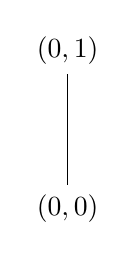
\begin{tikzpicture}
                \node (max) at (2,2) {$(0,1)$};
                \node (min) at (2,0) {$(0,0)$};

                \draw (min) -- (max);
                \draw[preaction={draw=white, -,line width=6pt}] (min) -- (max);
            \end{tikzpicture}
                                        &
            \begin{tikzpicture}
                \node (max) at (0,4) {$(1,1)$};
                \node (a) at (-2,2) {$(1,0)$};
                \node (b) at (2,2) {$(0,1)$};
                \node (min) at (0,0) {$(0,0)$};

                \draw (min) -- (a) -- (max) -- (b);
                \draw[preaction={draw=white, -,line width=6pt}] (a) -- (min) -- (b);
            \end{tikzpicture}
                                        &
            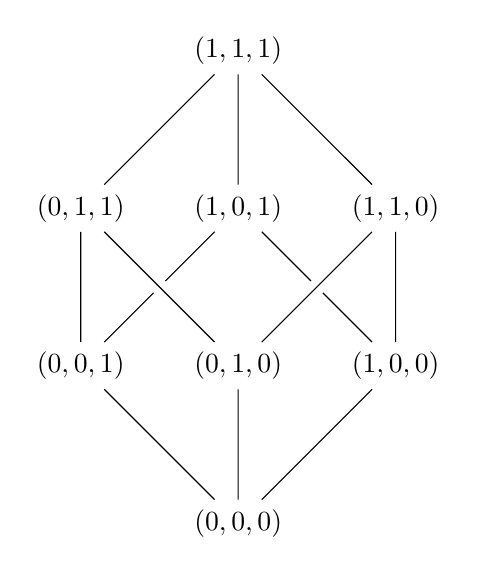
\begin{tikzpicture}
                \node (max) at (0,4) {$(1,1,1)$};
                \node (a) at (-2,2) {$(0,1,1)$};
                \node (b) at (0,2) {$(1,0,1)$};
                \node (c) at (2,2) {$(1,1,0)$};
                \node (d) at (-2,0) {$(0,0,1)$};
                \node (e) at (0,0) {$(0,1,0)$};
                \node (f) at (2,0) {$(1,0,0)$};
                \node (min) at (0,-2) {$(0,0,0)$};
                \draw (min) -- (d) -- (a) -- (max) -- (b) -- (f)
                (e) -- (min) -- (f) -- (c) -- (max)
                (d) -- (b);
                \draw[preaction={draw=white, -,line width=6pt}] (a) -- (e) -- (c);
            \end{tikzpicture}
            \\
            Diagrama Hasse $\mathbb{B}$ & \quad\quad\quad Diagrama Hasse $\mathbb{B}^2$ & \quad\quad\quad Diagrama Hasse $\mathbb{B}^3$
        \end{tabular}
    \end{center}
\end{ejemplo}
\smallskip
\begin{properties}
    Sea $(B, \lor, \land, \overline{\square}, 0, 1)$ un álgebra de Boole. Entonces $\forall x,y,z \in A$:
    \begin{itemize}
        \item $0 \leq x \leq 1$.
        \item Isotonía: Si $x \leq y$, entonces $x \lor z \leq y$ y $x \land z \leq y \land z$.
        \item $x\leq y \Longleftrightarrow \overline{y} \leq \overline{x} \Longleftrightarrow x \leq \overline{y} = 0$.
        \item $x \land y \leq z \Longleftrightarrow x \leq \overline{y} \lor z$.
    \end{itemize}
\end{properties}
\begin{ejemplo}
    Algunos ejemplos de álgebras de Boole a parte de los vistos anteriormente, destacar el álgebra de Boole de partes de un conjunto o el de divisores de $n$,
    $D_n$, bajo ciertas condiciones.
\end{ejemplo}

\begin{nprop}
    Sea $D_n$ los divisores de $n$. Si $n$ cumple que $\forall k > 1$, $k^2$ no divide a $n$, entonces todo $x \in D_n$ tiene complemento $\overline{x} = \frac{n}{x}$.
\end{nprop}
\begin{nprop}
    Sea $n \in \nat$, $n > 1$. $D_n$ es un álgebra de Boole si y sólo si $n$ es libre de cuadrados.
\end{nprop}
\begin{nota}
    Diremos que $n$ es libre de cuadrados cuando en su factorización como producto de números primos, todos tienen exponente 1.
\end{nota}

\subsection{Átomos de un Álgebra}
\begin{ndef}[Maximal y minimal]
    Sea $X$ un conjunto con una relación de orden $\leq$, y sea $m \in X$. Se dice que $m$ es un \textbf{elemento maximal de $X$}, si y sólo si, no existe $x \in X$ con $x \neq m$ tal que $m \leq x$.
    De manera análoga, $m$ es un \textbf{elemento minimal de $X$}, si y sólo si, no existe $x \in X$ con $m \neq x$ tal que $x \leq m$.
\end{ndef}
\begin{ndef}[Átomo]
    Sea $B$ un álgebra de Boole y $a \in B$. Se dice que $a$ es un \textbf{átomo} si $a$ es un elemento minimal de $B \setminus \{0\}$. Es decir,
    $\forall a \in B \setminus \{0\} \ (x \leq a \implies x = a)$. Denotaremos al conjunto que contiene a los átomos de B por $At(B)$.
\end{ndef}
\begin{ndef}[Coátomo]
    Sea $B$ un álgebra de Boole y $a \in B$ un átomo de $B$. Diremos entonces que $\overline{a}$ es un \textbf{coátomo}.
    Denotaremos al conjunto que contiene a los coátomos de B por $coAt(B)$.
\end{ndef}

\begin{nth}
    Sea $B$ un álgebra de Boole finita y $x \in X \setminus \{0\}$. Entonces $x$ se expresa de forma única como supremo de átomos.
\end{nth}
Este teorema tiene su versión dual que dice así:
\begin{nth}
    Sea $B$ un álgebra de Boole finita y $x \in X \setminus \{0\}$. Entonces $x$ se expresa de forma única como ínfimo de coátomos.
\end{nth}

\begin{lema}
    Sea $B$ un álgebra de Boole finita y $x \in X \setminus \{0\}$. Entonces existe $a \in B$ átomo tal que $a \leq x$.
\end{lema}
\begin{nota}
    Denotamos por $A_x$ al conjunto de elementos de $A$ menores o iguales que x.
\end{nota}

\begin{ejemplo}
    Los átomos de $\mathbb{B}^n$ son aquellos que tienen todas las coordenadas nulas menos una y sus coátomos son los elementos que tienen tan solo una coordenada nula.
\end{ejemplo}
\begin{ejemplo}
    Los átomos del álgebra de Boole de $\mathcal{P}(X)$ son los conjuntos unitarios.
\end{ejemplo}

\begin{ndef}[Álgebra de Boole atómica]
    Un álgebra de Boole $B$ es atómica si para todo $x \in B \setminus \{0\}$ existe un átomo $a$ tal que $a \leq x$.
\end{ndef}
\begin{nth}
    Todo álgebra de Boole finita es atómica.
\end{nth}
\begin{nth}
    En todo álgebra de Boole $B$ son equivalentes:
    \begin{enumerate}
        \item $a \in At(B)$
        \item $\forall x \in B, a \leq x \ o \ a \leq \overline{x}$
        \item $0 < a \ y \ \forall x,y \in B \ (a \leq x \lor y \Leftrightarrow a \leq x \ o \ a \leq y)$
    \end{enumerate}
\end{nth}
\begin{nth}
    Sea $B$ un álgebra de Boole finita  y $x \in B$, entonces $x = \bigvee \{a \in At(B): a \leq x\}$
\end{nth}
\begin{nth}
    Sea $B$ un álgebra de Boole finita  y $x \in B$, entonces $x = \bigwedge \{a \in coAt(B): a \leq x\}$
\end{nth}

\begin{ncor}
    Toda álgebra de Boole finita es isomorfa al álgebra de Boole de partes de sus átomos.
    \begin{center} $B \cong \mathcal{P} (At(B))$ \end{center}
\end{ncor}

\begin{ncor}
    Toda  álgebra de Boole finita B tiene $2^n$ elementos, donde $n$ es el número de átomos de $B$.
\end{ncor}

\begin{nth}
    Si dos álgebras de Boole finitas $A$, $B$ tienen el mismo número de elementos, entonces son isomorfas:
    \begin{center}
        $A \cong B$
    \end{center}
\end{nth}


\subsection{Funciones booleanas elementales}
\begin{ndef}[Función booleana]
    Una función booleana con $n$ variables es una aplicación $f: \mathbb{B}^n \rightarrow \mathbb{B}$.
    Denotaremos por $F_n$ al conjunto de las funciones booleanas con $n$ variables. Es decir,
    \begin{center}
        $F_n = \{f:\mathbb{B}^n \rightarrow \mathbb{B}, \ f$ es una aplicación$\}$
    \end{center}
\end{ndef}
\begin{ndef}[Puerta lógica]
    Una puerta lógica con $n$ entradas es una función booleana elemental de $n$ variables, es decir, un elemento del álgebra de Boole
    $F_n = Ap(\mathbb{B}^n, \mathbb{B})$.
\end{ndef}

\subsubsection{Funciones booleanas de una variable}
Para $n=1$, $f: \{0,1\} \rightarrow \{0,1\}$ tenemos 4 aplicaciones:
\begin{center}
    \begin{tabular}{ |c||c|c|c|c|  }
        \hline
        $x$ & $f_0^1$ & $f_1^1$ & $f_2^1$ & $f_3^1$ \\
        \hline
        0   & 0       & 0       & 1       & 1       \\
        1   & 0       & 1       & 0       & 1       \\
        \hline
    \end{tabular}
\end{center}

\begin{tabular}{ll}
    \tabitem \textbf{Función constante 0:} & $f_0^1(x)=0$            \\
    \tabitem \textbf{Función identidad:}   & $f_1^1(x)=x$            \\
    \tabitem \textbf{Función complemento:} & $f_2^1(x)=\overline{x}$ \\
    \tabitem \textbf{Función constante 1:} & $f_3^1(x)=1$            \\
\end{tabular}
\begin{nota}
    La función complemento \textbf{NOT} se representa en circuitos mediante la siguiente figura: \smallskip
    \begin{center}
        \begin{circuitikz}
            \draw (0,0) node[not port] (mynot) {};
        \end{circuitikz}
        \\ NOT
    \end{center}
\end{nota}

\subsubsection{Funciones booleanas de dos variables}
Para $n=2$, $f: \{0,1\} \rightarrow \{0,1\}$ tenemos 16 aplicaciones:
\begin{center}
    \begin{tabular}{ |c||c|c|c|c|c|c|c|c|c|c|c|c|c|c|c|c|  }
        \hline
        $x$   & $f_0^2$ & $f_1^2$ & $f_2^2$ & $f_3^2$ & $f_4^2$ & $f_5^2$ & $f_6^2$ & $f_7^2$ & $f_8^2$ & $f_9^2$ & $f_{10}^2$ & $f_{11}^2$ & $f_{12}^2$ & $f_{13}^2$ & $f_{14}^2$ & $f_{15}^2$ \\
        \hline
        (0,0) & 0       & 0       & 0       & 0       & 0       & 0       & 0       & 0       & 1       & 1       & 1          & 1          & 1          & 1          & 1          & 1          \\
        (0,1) & 0       & 0       & 0       & 0       & 1       & 1       & 1       & 1       & 0       & 0       & 0          & 0          & 1          & 1          & 1          & 1          \\
        (1,0) & 0       & 0       & 1       & 1       & 0       & 0       & 1       & 1       & 0       & 0       & 1          & 1          & 0          & 0          & 1          & 1          \\
        (1,1) & 0       & 1       & 0       & 1       & 0       & 1       & 0       & 1       & 0       & 1       & 0          & 1          & 0          & 1          & 0          & 1          \\
        \hline
    \end{tabular}
\end{center}

\begin{tabular}{ll}
    \tabitem \textbf{Función constante 0:}            & $f_0^2(x,y)=0$                                                     \\
    \tabitem \textbf{Función AND:}                    & $f_1^2(x,y)=x \cdot y$                                             \\
    \tabitem                                          & $f_2^2(x,y)=x \cdot \overline{y}$                                  \\
    \tabitem \textbf{Función proyección de x:}        & $f_3^2(x,y)=\pi_1(x,y) = x$                                        \\
    \tabitem                                          & $f_4^2(x,y)=\overline{x} \cdot y$                                  \\
    \tabitem \textbf{Función proyección de y:}        & $f_5^2(x,y)=\pi_2(x,y) = y$                                        \\
    \tabitem \textbf{Función XOR:}                    & $f_6^2(x,y)=x \oplus y$                                            \\
    \tabitem \textbf{Función OR:}                     & $f_7^2(x,y)=x + y$                                                 \\
    \tabitem \textbf{Función NOR:}                    & $f_8^2(x,y)=x \downarrow y = \overline{x} \cdot \overline{y}$      \\
    \tabitem \textbf{Función XNOR:}                   & $f_9^2(x,y)=x \leftrightarrow y = \overline{x} \cdot \overline{y}$ \\
    \tabitem \textbf{Función proyección negada de y:} & $f_{10}^2(x,y)=\overline{\pi}_2(x,y) = \overline{y}$               \\
    \tabitem                                          & $f_{11}^2(x,y)= x \leftarrow y$                                    \\
    \tabitem \textbf{Función proyección negada de x:} & $f_{12}^2(x,y)=\overline{\pi}_1(x,y) = \overline{x}$               \\
    \tabitem                                          & $f_{13}^2(x,y)= x \rightarrow y = \overline{x} + y$                \\
    \tabitem \textbf{Función NAND:}                   & $f_{14}^2(x,y)=x \uparrow y$                                       \\
    \tabitem \textbf{Función constante 1:}            & $f_{15}^2(x,y)=1$                                                  \\
\end{tabular}
\begin{nota}
    En electrónica, estas son las figuras para las siguientes puertas lógicas: \\
    \centering
    \begin{tabular}{llllll}
        \\
        \begin{circuitikz}
            \draw (0,0) node[and port] (myand) {};
        \end{circuitikz}
            &
        \begin{circuitikz}
            \draw (0,0) node[xor port] (myxor) {};
        \end{circuitikz}
            &
        \begin{circuitikz}
            \draw (0,0) node[or port] (myor) {};
        \end{circuitikz}
            &
        \begin{circuitikz}
            \draw (0,0) node[nor port] (mynor) {};
        \end{circuitikz}
            &
        \begin{circuitikz}
            \draw (0,0) node[xnor port] (myxnor) {};
        \end{circuitikz}
            &
        \begin{circuitikz}
            \draw (0,0) node[nand port] (mynand) {};
        \end{circuitikz}
        \\
        AND & XOR & OR & NOR & XNOR & NAND
    \end{tabular}
\end{nota}

\subsection{Maneras de expresar una función}
\subsubsection{Expresiones booleanas}
Para listar las diferentes formas de dar una función booleana, usaremos el siguiente ejemplo en todos los casos: $\{f:\mathbb{B}^3 \rightarrow \mathbb{B} \ / \ f(x,y,z) = (\overline{x} \cdot y) + (\overline{y} \cdot z)\}$.
A esta manera de denominar una función booleana se le conoce como \textbf{expresión booleana}.
\begin{ndef}[Expresión booleana]
    Sea $X = \{x_1,x_2,\cdots,x_n\}$ un conjunto de variables. Se definen las expresiones booleanas sobre el conjunto $X$  de forma recursiva como sigue:
    \begin{enumerate}
        \item Si $x \in X \cup \{0,1\}$ entonces $x$ es una expresión booleana.
        \item Si $e_1,e_2$ son expresiones booleanas, entonces lo son $e_1+e_2, \ e_1 \cdot e_2$ y $\overline{e_1}$.
    \end{enumerate}
\end{ndef}
\begin{ndef}[Literal]
    Denominaremos literales a las expresiones booleanas que sean variables o sus complementos.
\end{ndef}
\begin{ndef}
    Dos expresiones booleanas son equivalentes si las correspondientes funciones booleanas son iguales. Si $e_1$ e $e_2$ son expresiones booleanas equivalentes emplearemos el símbolo $e_1=e_2$.
\end{ndef}
\begin{nprop}
    Sean $e_1,e_2, e_3$ expresiones booleanas en $n \in \nat$ variables. Entonces se cumple:

    \begin{tabular}{ll}
        \tabitem $e_1 + (e_2 + e_3) = (e_1 + e_2) + e_3$                        & $e_1 \cdot (e_2 \cdot e_3) = (e_1 \cdot e_2) \cdot e_3$      \\
        \tabitem $e_1 + e_2 = e_2 + e_1$                                        & $e_1 \cdot e_2 = e_2 \cdot e_1$                              \\
        \tabitem $e_1 + e_1 = e_1$                                              & $e_1 \cdot e_1 = e_1$                                        \\
        \tabitem $e_1 \cdot (e_2 + e_3) = e_1 \cdot e_2 + e_1 \cdot e_3$        & $e_1 + (e_2 \cdot e_3) = (e_1 + e_2) \cdot (e_1 + e_3)$      \\
        \tabitem   $\overline{e_1 + e_2} = \overline{e_1} \cdot \overline{e_2}$ & $\overline{e_1 \cdot e_2} = \overline{e_1} + \overline{e_2}$ \\
        \tabitem $e_1 + \overline{e_1} = 1$                                     & $e_1 \cdot \overline{e_1} = 0$                               \\
        \tabitem $e_1 + 1 = 1$                                                  & $e_1 \cdot 0 = 0$                                            \\
        \tabitem $e_1 + 0 = e_1$                                                & $e_1 \cdot 1 = e_1$                                          \\
        \tabitem $\overline{1} = 0$                                             & $\overline{0} = 1$                                           \\
    \end{tabular}
\end{nprop}

\subsubsection{Tablas de la verdad}
Podemos elaborar una tabla a partir de una función dada. Esta tabla se llama \textbf{tabla de la verdad}. En el caso de $f$, sería así:
\begin{center}
    \begin{tabular}{ |c|c|c||c|  }
        \hline
        $x$ & $y$ & $z$ & $f(x,y,z)$ \\
        \hline
        0   & 0   & 0   & 0          \\
        0   & 0   & 1   & 1          \\
        0   & 1   & 0   & 1          \\
        0   & 1   & 1   & 1          \\
        1   & 0   & 0   & 0          \\
        1   & 0   & 1   & 1          \\
        1   & 1   & 0   & 0          \\
        1   & 1   & 1   & 0          \\
        \hline
    \end{tabular}
\end{center}

\subsubsection{Enumeración}
Otra forma de dar dicha función es mencionando su número de variables y el número binario que forman. Este número, dado $r$, debe cumplir $0 \leq r < 2^{2^n}$.
En nuestro ejemplo, tendríamos que $2^6+2^5+2^4+2^2 = 116$. La llamaríamos la función 116 de tres variables.

\subsubsection{Mapas de Karnaugh}
Los mapas de Karnaugh son una disposición plana en forma de cuadrícula de la tabla de una función booleana quenos ayudará a obtener los implicantes primos y las formas no redundantes de la función.
El mapa de Karnaugh de $f$ sería:
\begin{center}
    \begin{Karnaugh_2x4}
        \minterms{1,4,5,6}
    \end{Karnaugh_2x4}
\end{center}

\subsection{Formas canónicas}
A la hora de identificar una expresión booleana, existen 2 métodos: la \textbf{forma canónica conjuntiva} y la \textbf{forma canónica disyuntiva}.
En el caso de la forma canónica disyuntiva, es necesario obtener las \textbf{conjunciones fundamentales} y para ello, definamos previamente varios conceptos:

Para la próxima definición, definimos las potencias de $a$ como $a^i = a^*$ si $i = *$, $a^i = 1$ si $i = 0$ y $a^i = a$ si $i = 1$:
\begin{ndef}[Conjunción fundamental o monomio]
    Una conjunción (fundamental) en $n$ variables es una expresión booleana de la forma $\mu = x_1^{e_1} \land x_2^{e_2} \land \cdots \land x_n^{e_n}$ donde $e_i \in \{0,1,\overline{\square}\}$. $\mu$ es una conjunción o monomio fundamental con elementos de $X$.
    El número de conjunciones fundamentales de $n$ variables distintas es $3^n$.
\end{ndef}

\begin{ndef}[Mintérmino]
    Una conjunción elemental o mintérmino en $n$ variables es una expresión booleana de la forma $m = x_1^{e_1} \land x_2^{e_2} \land \cdots \land x_n^{e_n}$ donde $e_i \in \{1,\overline{\square}\}$.
\end{ndef}
\begin{ndef}[Maxtérmino]
    Una disyunción elemental o maxtérmino en $n$ variables es una expresión booleana de la forma $M = x_1^{e_1} \lor x_2^{e_2} \lor \cdots \lor x_n^{e_n}$ donde $e_i \in \{0,\overline{\square}\}$.
\end{ndef}
\begin{nota}
    Es decir, los minterm son las funciones que valen 1 para una única combinación de valores de sus variables y los maxterm las que valen 0.
\end{nota}
El número de mintérminos (y de maxtérminos) en $n$ variables es $2^n$.
\begin{ejemplo}[Visual]
    Tomemos las funciones conjunción de tres variables, por tanto hay $3^3 = 27$ conjunciones.
    De aquí, obtenemos todas las funciones posibles según el número de literales posibles: \\
    \begin{tabular}{ll}
        \tabitem \textbf{3 literales:} & $\overline{x} \cdot \overline{y}\cdot \overline{z}, \overline{x} \cdot \overline{y}\cdot z, \overline{x} \cdot y \cdot \overline{z}, x \cdot \overline{y} \cdot \overline{z}, \overline{x} \cdot y \cdot z, x \cdot \overline{y} \cdot z, x \cdot y \cdot \overline{z}, x \cdot y \cdot z$. \\
        \tabitem \textbf{2 literales:} & $\overline{x} \cdot \overline{y}, \overline{x} \cdot y, x \cdot \overline{y}, x \cdot y, \overline{x} \cdot \overline{z}, \overline{x} \cdot z, x \cdot \overline{z}, x \cdot z, \overline{y} \cdot \overline{z}, \overline{y} \cdot z, y \cdot \overline{z}, y \cdot z$.                   \\
        \tabitem \textbf{1 literal:}   & $\overline{x}, x, \overline{y}, y, \overline{z}, z$.                                                                                                                                                                                                                                        \\
        \tabitem \textbf{0 literales:} & 1
    \end{tabular}
    \begin{center}
        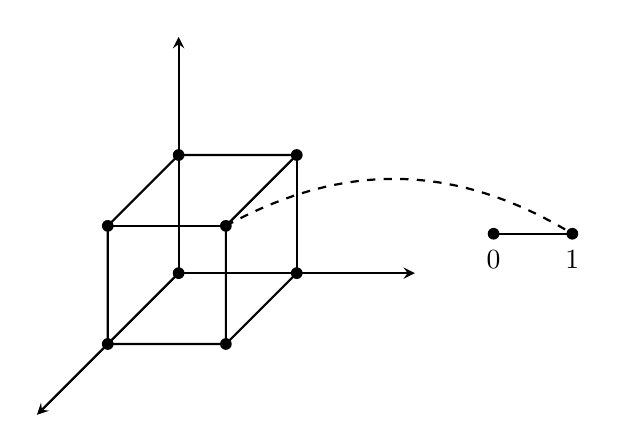
\begin{tikzpicture}[x=0.5cm,y=0.5cm,z=0.3cm,>=stealth,thick]
            % Ejes
            \draw[->] (xyz cs:x=0) -- (xyz cs:x=6) node[above] {};
            \draw[->] (xyz cs:y=0) -- (xyz cs:y=6) node[right] {};
            \draw[->] (xyz cs:z=0) -- (xyz cs:z=-6) node[above] {};

            % Líneas
            \draw[thick]
            (xyz cs:z=-3) --
            +(0,3) coordinate (u) --
            (xyz cs:y=3) --
            +(3,0) --
            ++(xyz cs:x=3,z=-3) coordinate (v) --
            +(0,-3) coordinate (w) --
            cycle;
            \draw[thick] (u) -- (v);
            \draw[thick] (3,0) -- (w);
            \draw[thick] (3,0) |- (0,3);
            \draw[thick] (8,1) -- (10,1);

            % Puntos
            \node[fill,circle,inner sep=1.5pt] at (xyz cs:z=-3) {};
            \node[fill,circle,inner sep=1.5pt] at (u) {};
            \node[fill,circle,inner sep=1.5pt] at (v) {};
            \node[fill,circle,inner sep=1.5pt] at (w) {};
            \node[fill,circle,inner sep=1.5pt] at (0,0) {};
            \node[fill,circle,inner sep=1.5pt] at (3,0) {};
            \node[fill,circle,inner sep=1.5pt] at (0,3) {};
            \node[fill,circle,inner sep=1.5pt] at (3,3) {};
            \node[fill,circle,inner sep=1.5pt, label={below:0}] at (8,1) {};
            \node[fill,circle,inner sep=1.5pt, label={below:1}] at (10,1) {};
            % Aplicación
            \draw [dashed] (v) to[bend left] node {} (10,1);
        \end{tikzpicture}
    \end{center}

    Como podemos ver en ésta representación gráfica, en el caso dado podemos apreciar que la función booleana definida por un mintérmino aplica un vértice del n-cubo en el 1 y el resto en el 0.
    En el caso de 2 literales, aplica una arista (2 vértices) al 1 y el resto al 0. En el caso de 1 literal, aplica una cara (4 vértices) en el uno, etc.
\end{ejemplo}

A partir del ejemplo deducimos que si faltan $r$ variables, se aplican $2^r$ vértices contiguos, denominados \textbf{hipercaras de dimensión $r$}, en el 1. El número de conjunciones
hipercaras de dimensión $r$ es $\binom{n}{n-r} \cdot 2^{n-r}$.
\begin{nota}
    $\mu_1 < \mu_2$ si, y sólo si, $\mu_2$ se obtiene suprimiendo literales de $\mu_1$.
\end{nota}

\begin{ejemplo}
    Estas conjunciones se pueden representar fácilmente en un mapa de Karnaugh. Veamos la representación de las conjunciones de 3 variables $\overline{x} \cdot z$ (arista) y $x$ (cara):
    \begin{center}
        \begin{Karnaugh_2x4}
            \minterms{2,3,4,5,6,7}
            \implicant{3}{6}{green}
            \implicant{4}{5}{}
        \end{Karnaugh_2x4}
    \end{center}
\end{ejemplo}

\subsubsection{Forma canónica disyuntiva}
\begin{ndef}
    Una forma disyuntiva es una suma de conjunciones.
\end{ndef}
\begin{nth}
    Los mintérminos (conjunciones elementales) son los átomos del álgebra de Boole $F_n$.
\end{nth}
\begin{nth}[de la forma canónica disyuntiva]
    Toda función booleana elemental se puede expresar de forma única como suma (disyunción, supremo) de mintérminos.
\end{nth}
\begin{ncor}
    Toda función booleana elemental se puede expresar como suma de conjunciones.
\end{ncor}
El número de formas disyuntivas expresados de manera similar a los polinomios es de $2^{3^n}$, que dividido entre el número de funciones elementales $2^{2^n}$, nos da un promedio de $2^{3^n-2^n}$ formas disyuntivas para una determinada función.
De entre ellas, la que nos interesa es la canónica.

\subsubsection{Algoritmo de la forma canónica disyuntiva}
El algoritmo consta de los siguientes pasos:
\begin{enumerate}
    \item Partimos de una expresión booleana de la función.
    \item Mediante las leyes de De Morgan y la ley de doble complemento interiorizamos el complemento ($\overline{\square}$) hasta que sólo afecte a las variables.
    \item Distribuimos el producto (ínfimo) sobre la suma (supremo) hasta que nos quede una suma de conjunciones fundamentales.
    \item (Optativo) Simplificamos las expresión por absorción de conjunciones fundamentales.
    \item Hacemos uso de la igualdad $\mu = \mu \cdot 1 = \mu \cdot (x + \overline{x}) = \mu \cdot x + \mu \cdot \overline{x}$ para lograr que todas las variables aparezcan en todos los monomios de la expresión. Partiendo de la forma disyuntiva obtenida
          seleccionamos un monomio en el que falte una variable y lo sustituimos por la suma de dos monomios donde ya faltará una variable menos.
    \item Cuando todos los monomios sean mintérminos, eliminamos repeticiones por idempotencia y obtenemos la forma canónica disyuntiva.
\end{enumerate}
Otra manera más sencilla de llegar a la misma solución es mediante el \textbf{método de la tabla}, donde para cada fila de la función que vale 1, escribimos el mintérmino asociado.
\begin{ejemplo}
    Apliquemos el algoritmo con $f(x,y,z) = xy \cdot (\overline{z} + y)$: \\
    $f(x,y,z) = xy \cdot (\overline{z} + y) = xy\overline{z} + xy = xy\overline{z} + xyz + xy\overline{z} = xy\overline{z} + xyz = m_6 + m_7$
    Ahora, si usamos el método de la tabla, veremos que obtenemos la misma solución:
    \begin{center}
        \begin{tabular}{ |c|c|c||c|  }
            \hline
            $x$ & $y$ & $z$ & $f(x,y,z)$ \\
            \hline
            0   & 0   & 0   & 0          \\
            0   & 0   & 1   & 0          \\
            0   & 1   & 0   & 0          \\
            0   & 1   & 1   & 0          \\
            1   & 0   & 0   & 0          \\
            1   & 0   & 1   & 0          \\
            1   & 1   & 0   & 1          \\
            1   & 1   & 1   & 1          \\
            \hline
        \end{tabular}
    \end{center}
    \centering $f(x,y,z) = xy \cdot (\overline{z}+y) = m_6 + m_7 = xy\overline{z} + xyz$
\end{ejemplo}
Sin embargo, aunque la forma canónica resulte interesante de obtener, luego en la práctica no suele ser la manera más óptima, lo que nos llevará a buscar simplificaciones.

\subsubsection{Forma canónica conjuntiva}
De manera similar a la forma canónica disyuntiva, tenemos por dualidad que:
\begin{ndef}
    Una forma conjuntiva es un producto de disyunciones.
\end{ndef}
\begin{nth}
    Los maxtérminos (disyunciones elementales) son los coátomos del álgebra de Boole $F_n$.
\end{nth}
\begin{nth}[de la forma canónica conjuntiva]
    Toda función booleana elemental se puede expresar de forma única como producto (conjunción, ínfimo) de maxtérminos.
\end{nth}
\begin{ncor}
    Toda función booleana elemental se puede expresar como producto de disyunciones.
\end{ncor}

\subsection{Simplificación}
Como hemos dicho antes, muchas veces nos va a interesar obtener una simplificación de ésta forma canónica disyuntiva. Para ello aplicaremos dos reglas:
\begin{itemize}
    \item \textbf{Eliminación de un monomio.} Si $f = \mu + R = R$, entonces podemos eliminar $\mu \Longleftrightarrow \mu R = \mu$ .
    \item \textbf{Eliminación de un literal en un monomio.} Si $f = \mu + R = \mu ' + R$, podemos sustituir $\mu$ por $\mu ' \Longleftrightarrow \mu < \mu ' \Longleftrightarrow \mu ' f = \mu '$.
\end{itemize}
A este proceso lo llamremos \textbf{simplificación}. A las formas disyuntivas que no la admitan las llamaremos \textbf{formas disyuntivas no redundantes, irredundantes o no simplificables}.

\subsubsection{Algoritmo de simplificación}
Se parte de una forma disyuntiva arbitraria de la función. Se ordenan los monomios y dentro de los monomios se ordenan los literales y aplicamos las siguientes reglas a cada uno de los monomios en el orden dado.
\begin{enumerate}
    \item Se intenta suprimir el monomio correspondiente viendo si es menor que otro de los que intervienen en la forma.
    \item Si no se suprime el monomio se prueba a suprimir los literales del monomio en el orden dado.
    \item Cuando no se pueda simplificar más se pasa al monomio siguiente.
\end{enumerate}
\begin{ejemplo}
    Apliquemos el algoritmo a $f(x,y,z) =\overline{x}\overline{y}\overline{z}+z\overline{x}\overline{y}+y\overline{x}z+xyz+\overline{z}xy+x\overline{y}\overline{z}$:
    \begin{center}
        \begin{tabular}{ |c|c|c|  }
            \hline
            Forma disyuntiva                                                                                                             & Conjunción                             & Operación                        \\
            \hline
            $\overline{x}\overline{y}\overline{z}+z\overline{x}\overline{y}+y\overline{x}z+xyz+\overline{z}xy+x\overline{y}\overline{z}$ & $\overline{x}\overline{y}\overline{z}$ & $sup(\overline{x})$              \\
            $\overline{y}\overline{z}+z\overline{x}\overline{y}+y\overline{x}z+xyz+\overline{z}xy+x\overline{y}\overline{z}$             & $z\overline{x}\overline{y}$            & $sup(z)$                         \\
            $\overline{y}\overline{z}+\overline{x}\overline{y}+y\overline{x}z+xyz+\overline{z}xy+x\overline{y}\overline{z}$              & $y\overline{x}\overline{z}$            & $sup(y)$                         \\
            $\overline{y}\overline{z}+\overline{x}\overline{y}+\overline{x}z+xyz+\overline{z}xy+x\overline{y}\overline{z}$               & $xyz$                                  & $sup(x)$                         \\
            $\overline{y}\overline{z}+\overline{x}\overline{y}+\overline{x}z+yz+\overline{z}xy+x\overline{y}\overline{z}$                & $\overline{z}xy$                       & $sup(\overline{z})$              \\
            $\overline{y}\overline{z}+\overline{x}\overline{y}+\overline{x}z+yz+xy+x\overline{y}\overline{z}$                            & $x\overline{y}\overline{z}$            & $sup(x\overline{y}\overline{z})$ \\
            $\overline{y}\overline{z}+\overline{x}\overline{y}+\overline{x}z+yz+xy$                                                      &                                        &                                  \\
            Segunda pasada                                                                                                               &                                        &                                  \\
            $\overline{y}\overline{z}+\overline{x}\overline{y}+\overline{x}z+yz+xy$                                                      & $\overline{x}\overline{y}$             & $sup(\overline{x}\overline{y})$  \\
            $\overline{y}\overline{z}+\overline{x}z+yz+xy$                                                                               & $yz$                                   & $sup(yz)$                        \\
            $\overline{y}\overline{z}+\overline{x}z+xy$                                                                                  &                                        &                                  \\
            \hline
        \end{tabular}
    \end{center}
    Donde la forma no redundante es $f(x,y,z) =\overline{y}\overline{z}+\overline{x}z+xy$.
    \begin{nota}
        El suprarayado $\overline{\square}$ se está aplicando de manera individual a cada variable.
    \end{nota}
    \begin{obs}
        El orden de los monomios y factores altera la forma no redundante obtenida.
    \end{obs}
\end{ejemplo}
\smallskip
\begin{ndef}[Implicante]
    Un implicante de una función es un monomio fundamental que es menor o igual que la función.
\end{ndef}

\begin{ndef}[Implicante primo, simple o maximal]
    Un implicante primo de una función es un implicante de la función en el que al suprimir un literal deja de ser implicante.
\end{ndef}

\begin{ndef}[Implicante primo esencial]
    Un implicante primo esencial es aquel que contiene mintérminos 1 no contenidos dentro de ningún otro implicante primo.
\end{ndef}

\begin{nota}
    Todos los implicantes que aparecen en una forma disyuntiva no redundante son implicantes primos.
\end{nota}

\subsection{Forma reducida}
Como hemos visto, nos interesa obtener una forma más reducida que la canónica y para ello deberemos encontrar todos los implicantes primos y así encontrar la forma reducida más óptima para la medida considerada.
\begin{ndef}[Forma reducida]
    Llamamos forma disyuntiva reducida de una función a la suma de sus implicantes maximales.
\end{ndef}
\begin{nth}
    La suma de todos los implicantes primos de una función es una forma disyuntiva de la función.
\end{nth}

\subsubsection{Algoritmo de Quine para la obtención de los implicantes primos}
Se parte de la forma canónica disyuntiva (suma de mintérminos). Presenta la ventaja de poderse aplicar a cualquier número de generadores y ser programable, sin embargo, es pesado de llevar a cabo.
\begin{enumerate}
    \item Se clasifican los mintérminos según el número de variables que aparecen complementadas.
    \item En cada paso intentamos encontrar dos monomios en grupos adyacentes que difieran en un literal solamente
          (todas las variables excepto una con igual exponente) y que dan lugar a otro monomio sin el literal considerado,
          es decir, a partir de $x\mu$ y $\overline{x}\mu$ generamos $\mu$, siendo $x$ cualquier variable. La disposición hace que sólo se compare
          cada monomio con todos los del grupo siguiente de todas las formas posibles. Los que se agrupan se marcan
          con un aspa y a los que dan lugar se ponen en otra tabla. De esta forma los monomios en los que faltan una
          variable estarán en la tabla segunda.
    \item A continuación tenemos que comparar los monomios de la segunda tabla entre sí. Obteniendo la tabla siguiente con monomios en los que faltan dos variables y agrupados por numero de variables complementadas.
    \item Al finalizar, los monomios que no estén marcados no pueden ser menores que otros y por tanto estos serán los implicantes maximales o primos.
\end{enumerate}

\begin{ejemplo}
    Tomemos la función $f(x,y,z) =\overline{x} \cdot \overline{y} \cdot \overline{z}+\overline{x} \cdot y\overline{z}+x\overline{y} \cdot \overline{z}+xy\overline{z}+xyz$ y simplifiquémosla con el algoritmo de Quine:
    \begin{center}
        \begin{tabular}{lll}
            \begin{tabular}{ |c||c|  }
                \hline
                $\bullet$ & $\overline{x} \cdot \overline{y} \cdot \overline{z}$ \\
                \hline
                $\bullet$ & $\overline{x} \cdot y\overline{z}$                   \\
                $\bullet$ & $x\overline{y} \cdot \overline{z}$                   \\
                \hline
                $\bullet$ & $xy\overline{z}$                                     \\
                \hline
                $\bullet$ & $xyz$                                                \\
                \hline
            \end{tabular}

            \begin{tabular}{ |c||c|  }
                \hline
                $\bullet$ & $\overline{x} \cdot \overline{z}$ \\
                $\bullet$ & $\overline{y} \cdot \overline{z}$ \\
                \hline
                $\bullet$ & $y\overline{z}$                   \\
                $\bullet$ & $x\overline{z}$                   \\
                \hline
                          & $xy$                              \\
                \hline
            \end{tabular}

            \begin{tabular}{|c||c|}
                \hline
                 & $\overline{z}$ \\
                \hline
            \end{tabular}
        \end{tabular}
    \end{center}
    Tomando finalmente los monomios sin marcar, nos queda que la forma reducida de $f(x,y,z) = xy + \overline{z}$.
\end{ejemplo}

\subsubsection{Mapas de Karnaugh}
Este método consiste en buscar los implicantes primos a ojo mediante agrupaciones de unos contiguos. Para ello, buscaremos las hipercaras y tras ellas, variedades de orden inferior de manera descendente.
\begin{ejemplo}
    Tomemos $f(x,y,z) =\overline{x} \cdot \overline{y} \cdot \overline{z}+\overline{x} \cdot \overline{y} \cdot z+\overline{x} \cdot y \cdot z+x\overline{y} \cdot \overline{z}+x \cdot y\overline{z}+x \cdot y \cdot z=m_0+m_1+m_3+m_4+m_6+m_7$
    \begin{center}
        \begin{Karnaugh_2x4}
            \minterms{0,1,3,4,6,7}
            \implicant{0}{4}{green}
            \implicant{7}{6}{green}
            \implicant{3}{7}{green}
            \implicant{1}{3}{green}
            \implicant{0}{1}{green}
            \implicantsides{4}{6}{green}
        \end{Karnaugh_2x4}
    \end{center}
    Por tanto, $f(x,y,z) = \overline{x} \cdot \overline{y} + \overline{x} \cdot z + y \cdot z + x \cdot y + x \cdot \overline{z} + \overline{y} \cdot \overline{z}$
\end{ejemplo}

\subsubsection{Método de los consensos}
Se parte de cualquier forma disyuntiva de la función y está basado en la siguiente igualdad del álgebra de Boole: $x\mu_1 + \overline{x}\mu_2 = x\mu_1 + \overline{x}\mu_2 + \mu_1\mu_2$, siendo $x$ cualquier variable.
Al monomio $\mu_1\mu_2$ se le llama \textbf{consenso en $x$} de los monomios $x\mu_1$ y $x\mu_2$. \smallskip
Partiendo de cualquier forma disyuntiva, se van añadiendo los consensos en todas las variables de todas las parejas de monomios posibles (incluidos los que van apareciendo) y simplificando por absorción (monomios incluidos en otros).
Cuando no aparecen más consensos y se han hecho todas las absorciones, se obtiene la forma normal reducida, que es la suma de todos los implicantes maximales.
\begin{ejemplo}
    Aplicando el método de los consensos a $f(x,y,z) =\overline{x} \cdot \overline{y} \cdot \overline{z}+\overline{x} \cdot \overline{y} \cdot z+\overline{x} \cdot yz+x\overline{y} \cdot \overline{z}+xy\overline{z}+xyz$, tenemos que: \smallskip
    \begin{center}
        $f(x,y,z) =\overline{x} \cdot \overline{y} \cdot \overline{z}+\overline{x} \cdot \overline{y} \cdot z+\overline{x} \cdot yz+x\overline{y} \cdot \overline{z}+xy\overline{z}+xyz$ \\
        $= \overline{x} \cdot \overline{y} \cdot \overline{z}+\overline{x} \cdot \overline{y} \cdot z+\overline{x} \cdot yz+x\overline{y} \cdot \overline{z}+xy\overline{z}+xyz+\overline{x} \cdot \overline{y}$ \\
        $=\overline{x} \cdot yz+x\overline{y} \cdot \overline{z}+xy\overline{z}+xyz+\overline{x} \cdot \overline{y} \cdot $ \\
        $=\overline{x} \cdot yz+x\overline{y} \cdot \overline{z}+xy\overline{z}+xyz+\overline{x} \cdot \overline{y} \cdot +yz$ \\
        $= x\overline{y} \cdot \overline{z}+xy\overline{z}+\overline{x} \cdot \overline{y} \cdot +yz$ \\
        $=x\overline{y} \cdot \overline{z}+xy\overline{z}+\overline{x} \cdot \overline{y} \cdot +yz+x\overline{z}$ \\
        $=\overline{x} \cdot \overline{y} +yz+x\overline{z}$ \\
        $=\overline{x} \cdot \overline{y} +yz+x\overline{z}+\overline{x} \cdot z$ \\
        $=\overline{x} \cdot \overline{y} +yz+x\overline{z}+\overline{x} \cdot z+\overline{y} \cdot \overline{z}$ \\
        $=\overline{x} \cdot \overline{y} +yz+x\overline{z}+\overline{x} \cdot z+\overline{y} \cdot \overline{z}+xy$
    \end{center}
\end{ejemplo}

\subsubsection{Método de la forma canónica conjuntiva o producto de maxtérminos}
Se halla la forma canónica conjuntiva. Se distribuye el producto sobre la suma y se realizan todas las absorciones con lo que se obtiene la forma canónica reducida.
\begin{ejemplo}
    Habiendo obtenido los mintérminos de la función, supongamos el caso de $f(x,y,z) =m_0+m_2+m_3+m_6+m_7$. Por tanto, sacamos los maxtérminos y obtenemos que: \\
    $f(x,y,z) =M_1M_4M_5 = (x+y+\overline{z})(\overline{x} \cdot +y+z)(\overline{x} +y+\overline{z})= (xy+xz+\overline{x}y+y+yz+\overline{x} \cdot \overline{z}+y\overline{z})(\overline{x} \cdot +y+\overline{z})= (xz+y+\overline{x} \cdot \overline{z})(\overline{x} +y+\overline{z})=xyz+\overline{x}y+y+y\overline{z}+\overline{x} \cdot \overline{z}+\overline{x}y \overline{z}+\overline{x} \cdot \overline{z}=y+\overline{x} \cdot \overline{z}$
\end{ejemplo}

\subsection{Formas no redundantes}
En la forma reducida, por ser todos los implicantes primos, no se puede simplificar con la segunda regla pero en general, sí se puede con la primera. Para obtenerla, usaremos la \textbf{cuadrícula de Mac-Cluskey} y el \textbf{algoritmo de Petrick}.
\subsubsection{Cuadrícula de Mac-Cluskey y algoritmo de Petrick}
A partir de los implicantes maximales de una función vamos a contruir todas las formas disyuntivas irredundantes.
\begin{enumerate}
    \item Reducir la tabla (Cuadrícula de Mac-Cluskey) de implicantes primos eliminando las filas de implicantes primos esenciales y las columnas correspondientes.
    \item Etiquetar las filas de la tabla de implicantes primos reducida $P_ {1}, P_ {2}, P_ {3}, P_ {4}$, etc.
    \item Formar una función lógica que sea verdadera cuando se cubran todas las columnas. P consiste en un producto de sumas donde cada término de suma tiene la forma, donde cada uno representa una columna que cubre una fila. Es decir, $P = \prod_{i=0}^N(P _ {{i0}} + P _ {{i1}} +\cdots + P _ {{iN}})$.
    \item Reducir a la mínima suma de productos multiplicando y aplicando la ley de absorción. $X + XY = X$.
    \item Cada término del resultado representa una solución, es decir, un conjunto de filas que cubre todos los términos mínimos de la tabla. Para determinar las soluciones mínimas, primero encuentre aquellos términos que contengan un número mínimo de implicantes primos.
    \item Luego, para cada uno de los términos encontrados en el paso cinco, cuente el número de literales en cada implicante principal y encuentre el número total de literales.
    \item Elegir el término o términos compuestos por el número total mínimo de literales y escribir las sumas correspondientes de implicantes primos.
\end{enumerate}
\begin{ejemplo}
    Consideremos $f(x,y,z) =\overline{x} \cdot \overline{y} \cdot \overline{z}+\overline{x} \cdot \overline{y} \cdot z+\overline{x} \cdot yz+x\overline{y} \cdot \overline{z}+xy\overline{z}+xyz$ y obtengamos su forma reducida:
    \begin{center} $f(x,y,z) =xy+x\overline{z}+\overline{x} \cdot \overline{y}+\overline{y} \cdot \overline{z}+\overline{x} \cdot z+yz$ \end{center}
    Ahora, formemos la cuadrícula de Mac-Cluskey:
    \begin{center}
        \begin{tabular}{ |c|c|c|c|c|c|c|c|  }
            \hline
              &                                   & $m_0$    & $m_1$    & $m_3$    & $m_4$    & $m_6$    & $m_7$    \\
            \hline
            A & $xy$                              &          &          &          &          & $\times$ & $\times$ \\
            \hline
            B & $x\overline{z}$                   &          &          &          & $\times$ & $\times$ &          \\
            \hline
            C & $\overline{x} \cdot \overline{y}$ & $\times$ & $\times$ &          &          &          &          \\
            \hline
            D & $\overline{y} \cdot \overline{z}$ & $\times$ &          &          & $\times$ &          &          \\
            \hline
            E & $\overline{x} z$                  &          & $\times$ & $\times$ &          &          &          \\
            \hline
            F & $\overline{y} \cdot \overline{z}$ &          &          & $\times$ &          &          & $\times$ \\
            \hline
        \end{tabular}
    \end{center}
    \smallskip
    No hay ningún \textbf{implicante esencial o nuclear} en la tabla, pues no hay ninguna columna que sólo tenga un aspa. En caso de haberlo, dicho implicante debería estar en toda forma irredundante.
    Para simplificar la notación y facilitar su comprensión, usaremos las letras por las que hemos definido los monomios. Dicho esto, vemos que:
    \begin{align*}
        m_0 \equiv C + D & \quad m_1 \equiv C + E \\
        m_3 \equiv E + F & \quad m_4 \equiv B + D \\
        m_6 \equiv A + B & \quad m_7 \equiv A + F
    \end{align*}
    Por tanto, $P = (C+D)(C+E)(E+F)(B+D)(A+B)(A+F)$, donde operando y simplificando obtenemos que $P = ABCE+BCF+ACDF+BDEF+ADE$.
    De aquí obtenemos cinco recubrimientos minimales y por tanto cinco formas disyuntivas irredundantes de las cuáles cogeremos las más óptimas por su longitud:
    \begin{center}
        $B+C+F=x\overline{z}+\overline{x} \cdot \overline{y}+yz$ \\ $A+D+E=xy+\overline{y} \cdot \overline{z}+\overline{x} \cdot z$
    \end{center}
    De estas dos usaremos la que más nos convenga en función de lo exigido.
\end{ejemplo}
\begin{nota}
    Aunque no se hayan usado a lo largo del tema, los siguientes dos términos son muy utilizados en el ámbito del álgebra de Boole y conviene conocerlos:
    \begin{itemize}
        \item \textbf{POS:} Producto de sumas \textit{(product of sums)}.
        \item \textbf{SOP:} Suma de productos (\textit{sum of products)}.
    \end{itemize}
\end{nota}

\newpage
\section{Grafos}
\subsection{Introducción a la teoría de grafos}
En 1736, surgió el denominado \textit{problema de los puentes de Königsberg}. En aquella época, la ciudad de Königsberg estaba dividida en cuatro zonas por el río Pregel.
También habían siete puentes que comunicaban dichas regiones conforme aparece en la primera imagen:
\begin{center} 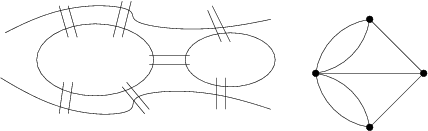
\includegraphics[scale=0.75]{konigsberg} \end{center}
El problema planteaba si sería posible cruzar por todos los puentes una sóla vez y volver al punto de partida.
De esta manera, \textbf{Leonhard Euler} dió con la solución, dando lugar a una nueva teoría en las matemáticas. Para ello, representó las zonas con cuatro puntos y los puentes como siete aristas, tal y como se contempla en la segunda imagen.
Sería así cómo se originaría la \textbf{teoría de grafos}.

\begin{ndef}[Grafo]
    Un \textbf{grafo} $G$ es un par $(V, E)$, donde $V$ y $E$ son conjuntos, junto con una aplicación $\gamma_G : E \rightarrow \{\{u,v\} : u,v \in V\}$.
    Al conjunto $V$ se le llama conjunto de vértices; al conjunto $E$ conjunto de lados o aristas, y a la aplicación $\gamma_G$ (o simplemente $\gamma$) aplicación de incidencia.
\end{ndef}
\begin{nota}
    También se le llama \textit{orden} al cardinal del conjunto de vértices $V$ y \textit{tamaño} al cardinal del conjunto de aristas  $E$.
\end{nota}

\begin{ndef}[Digrafo]
    Un \textbf{grafo dirigido, orientado o digrafo} es un par $(V,E)$, donde $V$ y $E$ son conjuntos, junto con dos aplicaciones $s,t : E \rightarrow V$. Las aplicaciones $s$ y $t$ se denominan respectivamente \textbf{aplicaciones dominio} y \textbf{aplicaciones codominio} \textit{("source" \& "target")}.
\end{ndef}

\begin{ndef}[Subgrafo]
    Sea $G = (V,E)$ un grafo con aplicación de incidencia $\gamma_G$. Un \textbf{subgrafo} $G'$ de $G$ es un nuevo grafo $G'=(V',E')$ donde $V' \subseteq V, \ E' \subseteq E$ y se verifica que $\gamma_{G'}(e) = \gamma_G(e)$ para cualquier $e \in E'$.
\end{ndef}

\begin{ndef}[Subgrafo completo]
    Sea $G' = (V', E')$ es un subgrafo de $G = (V, E)$, diremos que $G'$ es un \textbf{subgrafo completo} si dado $e \in E$ tal que $\gamma_G(e) \subseteq V'$, se verifica que $e \in E'$. Es decir, si tiene todos los lados que tenía $G$ y que unen vértices de $V'$.
\end{ndef}
\begin{obs}
    Un subgrafo completo está completamente determinado por el conjunto de vértices.
\end{obs}

A la hora de trabajar con grafos, diremos que dos lados $e_1$ y $e_2$ son \textbf{paralelos} si $\gamma_G(e_1) = \gamma_G(e_2)$. Un lado tal que $\gamma_G(e) = \{v\}$ se dice que es un \textbf{lazo}.
También se suelen nombrar los grafos que excluyen estos elementos como \textbf{grafos simples} y los grafos que hemos definido en 3.1 (que incluyen estos elementos) como \textbf{multigrafos}.

\begin{ndef}
    Sea $G$ un grafo. Un \textbf{camino} de longitud $n$ es una sucesión de lados $e_1 e_2 \cdots e_n$, junto con una sucesión de vértices $v_1 v_2 \cdots v_n$ tales que $\gamma_G(e_i) = \{v_{i-1},v_i\}$.
\end{ndef}

Veamos los distintos tipos de caminos que hay con ayuda de la siguiente tabla:
\begin{center}
    \begin{tabular}{|c|c|c|c|}
        \hline
        Nombre         & Vértices repetidos & Aristas repetidas & Abierto \\
        \hline
        Camino         & -                  & -                 & -       \\
        Camino cerrado & -                  & -                 & No      \\
        Recorrido      & -                  & No                & -       \\
        Camino simple  & No                 & No                & -       \\
        Circuito       & -                  & No                & No      \\
        Ciclo          & No                 & No                & No      \\
        \hline
    \end{tabular}
\end{center}
Consideraremos camino de longitud cero de $v$ a $v$ aquel cuya sucesión de vértices es $v$ y cuya sucesión de lados es vacía.

\begin{nprop}
    Sea $G$ un grafo. Supongamos que existe un camino de $u$ a $v$. Entonces existe un camino simple de $u$ a $v$.
\end{nprop}

\begin{nprop}
    Sea $G$ un grafo y sean $u$ y $v$ dos vértices distintos. Supongamos que tenemos dos caminos simples distintos de $u$ a $v$. Entonces existe un ciclo en $G$.
\end{nprop}

\begin{ndef}[Conexión]
    Sea $G$ un grafo. Se dice que $G$ \textbf{es conexo} si dados $u$ y $v$ dos vértices de $G$, existe al menos un camino de $u$ a $v$.
\end{ndef}
\begin{nota}
    La conexión por caminos en grafos establece una relación de equivalencia $R$. Un grafo \textbf{$G$ es conexo} si el conjunto cociente por $R$ tiene un solo elemento. Cada subgrafo completo determinado por los vértices de $R$ se denomina \textbf{componente conexa de $G$}.
\end{nota}

\subsection{Matrices asociadas a grafos}
\begin{ndef}
    Sea $G$ un grafo cuyo conjunto de vértices es $V = \{v_1,v_2,\cdots, v_n\}$. Se define su \textbf{matriz de adyacencia} como la matriz $A \in \mathcal{M} _n(\nat)$ cuyo coeficiente $(i,j)$ es igual al número de lados $e$ que unen $v_i$ con $v_j$, es decir, $f(e) = \{v_i,v_j\}$.
\end{ndef}

\begin{obs}
    De la anterior definición podemos sacar varias conclusiones:
    \begin{enumerate}
        \item Dicha matriz es simétrica.
        \item La matriz de adyacencia cambia según la ordenación de vértices tomada, siendo éstas matrices $A$ y $C$ semejantes entre sí a través de una matriz permutación $P$ tal que $P^{-1}CP=A$.
        \item La existencia de lados paralelos implica que existen coeficientes mayores que 1.
        \item En los grafos dirigidos, el coeficiente $a_{ij}$ es el número de lados que verifican que $s(e)=v_i$ y $t(e)=v_j$, no teniendo por qué ser simétrica.
        \item La matriz de adyacencia de un grafo determina a éste.
    \end{enumerate}
\end{obs}

\begin{nprop}
    Sea $G$ un grafo cuyo conjunto de vértices es $\{v_1,v_2,\cdots,v_n\}$ y sea $A$ su matriz de adyacencia. Entonces el coeficiente $(i,j)$ de $A^n$ es igual es igual al número de caminos de longitud $n$ que unen $v_i$ con $v_j$.
\end{nprop}

\begin{ndef}
    Sea $G$ un grafo cuyo conjunto de vértices es $V=\{v_1,v_2,\cdots,v_n\}$ y cuyo conjunto de lados es $E=\{e_1,e_2,\cdots,e_n\}$. Se define la \textbf{matriz de incidencia} de un grafo $G$ como la matriz $n \times m$ que tiene en la posición $(i,j)$ un 1 si $v_i \in \gamma_G(e_j)$ y 0 en otro caso.
\end{ndef}
\begin{obs}
    De la matriz de incidencia tenemos que:
    \begin{enumerate}
        \item Tomando otro orden de vértices y lados, la matriz de incidencia cambia. En este caso, ambas matrices $A$ y $C$ son equivalentes (de Tipo I), si podemos pasar de una a la otra mediante transformaciones elementales de manera que existen $P$ y $Q$ tal que $QCP=A$.
        \item Si un grafo tiene lados paralelos, esto se traduce en la matriz en forma de columnas iguales, mientras que los lazos se representan con valor de -1.
        \item Si el grafo es dirigido, el coeficiente $(i,j)$ puede valer -1 si el lado $e_i$ parte del vértice $v_i$. En este caso, el grafo no podrá tener lazos.
    \end{enumerate}
\end{obs}

\subsection{Isomorfismo de grafos}
\begin{ndef}
    Sean $G=(V,E)$ y $G'=(V',E')$ dos grafos con aplicaciones de incidencia $\gamma_G$ y $\gamma_{G'}$.
    Se dice que $G$ y $G'$ son isomorfos si existen dos biyecciones $h_V: V \rightarrow V'$ y $h_E:E \rightarrow E'$ tales que para cada
    lado $e \in E$ se verifica que $\gamma_G(h_E(e))=\{h_V(u), h_V(v)\}$ donde $\{u,v\}=\gamma_G(e)$.
    En tal caso diremos que las aplicaciones $h_V$ y $h_E$ forman un \textbf{isomorfismo} de $G$ a $G'$.
\end{ndef}

\begin{ndef}
    Una propiedad se dice invariante por isomorfismo si dados dos grafos isomorfos $G$ y $G'$, uno satisface la prpiedad si, y sólo si, la satisface el otro.
\end{ndef}

\begin{ndef}
    Sea $G$ un grafo y $v$ un vértice de $G$. Se define el grado de $v$, y lo denotaremos como $gr(v)$,
    como al número de lados (no lazos) de $G$ que son incidentes en $v$ más 2 veces el número de lazos incidentes en $v$.
    Denotaremos por $D_k(G)$ al número de vértices de $V$ que tienen grado igual a $k$. De la misma forma, llamaremos \textbf{sucesión de grados} a la sucesión $D_0(G), D_1(G), \cdots, D_k(G), \cdots$.
\end{ndef}

\subsection{Algunas familias de grafos}

\begin{ndef}[Grafo nulo]
    Denominaremos \textbf{grafo nulo} de orden $n$ al grafo $N_n$ que tiene por conjunto de vértices $\{v_1,v_1,\cdots,v_n\}$ y ninguna arista.
\end{ndef}
\begin{ejemplo} $N_1$, $N_3$ y $N_5$ respectivamente:
\begin{center}
    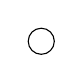
\begin{tikzpicture}[main/.style = {draw, circle}] 
        \node[main] (1) {}; 
    \end{tikzpicture}
    \quad\quad\quad\quad
    \begin{tikzpicture}[main/.style = {draw, circle}] 
        \node[main] (3) [below right of=1] {}; 
        \node[main] (4) [above right of=3] {}; 
        \node[main] (6) [below right of=4] {};
    \end{tikzpicture}
    \quad\quad\quad\quad
    \begin{tikzpicture}[main/.style = {draw, circle}] 
        \node[main] (2) [above right of=1] {};
        \node[main] (3) [below right of=1] {}; 
        \node[main] (4) [above right of=3] {};
        \node[main] (5) [above right of=4] {}; 
        \node[main] (6) [below right of=4] {};
    \end{tikzpicture}
\end{center}
\end{ejemplo}

\begin{ndef}[Grafo camino]
    Denominaremos \textbf{grafo camino} de orden $n$ al grafo \textbf{P$_n$} el cual tiene un único camino que pasa por todos sus vértices.
\end{ndef}
\begin{ejemplo} $P_1$, $P_3$ y $P_5$ respectivamente:
    \begin{center}
        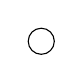
\begin{tikzpicture}[main/.style = {draw, circle}] 
            \node[main] (1) {}; 
        \end{tikzpicture}
        \quad\quad\quad\quad
        \begin{tikzpicture}[main/.style = {draw, circle}] 
            \node[main] (1) [below right of=1] {}; 
            \node[main] (2) [above right of=3] {}; 
            \node[main] (3) [below right of=4] {};
            \draw (1) -- (2) -- (3);
        \end{tikzpicture}
        \quad\quad\quad\quad
        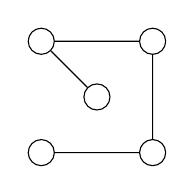
\begin{tikzpicture}[main/.style = {draw, circle}] 
            \node[main] (1) {};
            \node[main] (2) [above left of=1] {}; 
            \node[main] (3) [above right of=1] {};
            \node[main] (4) [below right of=1] {}; 
            \node[main] (5) [below left of=1] {};
            \draw (1) -- (2) -- (3) -- (4) -- (5);
        \end{tikzpicture}
    \end{center}
\end{ejemplo}

\begin{ndef}[Grafo regular]
    Diremos que un \textbf{grafo regular} es aquel en el cual todos los vértices tienen el mismo grado.
\end{ndef}

\begin{ndef}[Grafo circular]
    \textbf{Grafo circular o poligonal} \textbf{C$_n$}. Determinado por los vértices de un polígono regular. Los lados son los del polígono.
\end{ndef}
\begin{ejemplo} $P_3$ y $P_5$ respectivamente:
    \begin{center}
        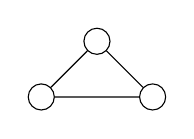
\begin{tikzpicture}[main/.style = {draw, circle}] 
            \node[main] (1) {}; 
            \node[main] (2) [below left of=1] {}; 
            \node[main] (3) [below right of=1] {};
            \draw (1) -- (2) -- (3) -- (1);
        \end{tikzpicture}
        \quad\quad\quad\quad
        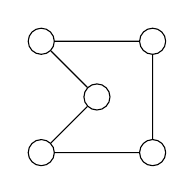
\begin{tikzpicture}[main/.style = {draw, circle}] 
            \node[main] (1) {};
            \node[main] (2) [above left of=1] {}; 
            \node[main] (3) [above right of=1] {};
            \node[main] (4) [below right of=1] {}; 
            \node[main] (5) [below left of=1] {};
            \draw (1) -- (2) -- (3) -- (4) -- (5) -- (1);
        \end{tikzpicture}
    \end{center}
\end{ejemplo}

\begin{ndef}[Grafo completo]
    Un \textbf{grafo completo} \textbf{K$_n$} es un grafo simple donde cada par de vértices está conectado por una arista. 
\end{ndef}
\begin{ejemplo} $P_4$ y $P_5$ respectivamente:
    \begin{center}
        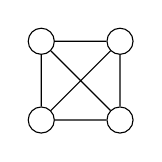
\begin{tikzpicture}[main/.style = {draw, circle}] 
            \node[main] (1) {}; 
            \node[main] (2) [left of=1] {}; 
            \node[main] (3) [below of=2] {};
            \node[main] (4) [below of=1] {};
            \draw (1) -- (2) -- (3) -- (4) -- (1) -- (3) -- (2) -- (4);
        \end{tikzpicture}
        \quad\quad\quad\quad
        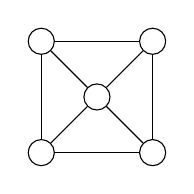
\begin{tikzpicture}[main/.style = {draw, circle}] 
            \node[main] (1) {};
            \node[main] (2) [above left of=1] {}; 
            \node[main] (3) [above right of=1] {};
            \node[main] (4) [below right of=1] {}; 
            \node[main] (5) [below left of=1] {};
            \draw (2) -- (3) -- (4) -- (5) -- (2);
            \draw (1) -- (2);
            \draw (1) -- (3);
            \draw (1) -- (4);
            \draw (1) -- (5);
        \end{tikzpicture}
    \end{center}
\end{ejemplo}

\begin{ndef}[Grafo estrella]
    Un \textbf{grafo estrella} \textbf{S$_n$} = \textbf{K$_{1,n}$} está determinado por los vértices de un polígono regular y su centro. Los lados son losque unen el centro con cada uno de los vértices del polígono.
\end{ndef}
\begin{ejemplo} $S_3$ y $S_4$ respectivamente:
    \begin{center}
        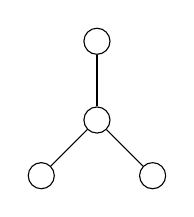
\begin{tikzpicture}[main/.style = {draw, circle}] 
            \node[main] (1) {}; 
            \node[main] (2) [above of=1] {}; 
            \node[main] (3) [below left of=1] {};
            \node[main] (4) [below right of=1] {};
            \draw (1) -- (2);
            \draw (1) -- (3);
            \draw (1) -- (4);
        \end{tikzpicture}
        \quad\quad\quad\quad
        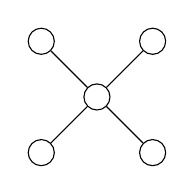
\begin{tikzpicture}[main/.style = {draw, circle}] 
            \node[main] (1) {};
            \node[main] (2) [above left of=1] {}; 
            \node[main] (3) [above right of=1] {};
            \node[main] (4) [below right of=1] {}; 
            \node[main] (5) [below left of=1] {};
            \draw (1) -- (2);
            \draw (1) -- (3);
            \draw (1) -- (4);
            \draw (1) -- (5);
        \end{tikzpicture}
    \end{center}
\end{ejemplo}

\begin{ndef}[Grafo rueda]
    Grafo rueda \textbf{W$_n$}. Determinado por los vértices de un polígono regular y su centro. Los lados son los del polígono y los que unen el centro con cada uno de los vértices del polígono.
\end{ndef}
\begin{ejemplo} $W_4$ y $W_5$ respectivamente:
    \begin{center}
        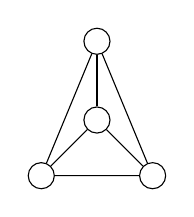
\begin{tikzpicture}[main/.style = {draw, circle}] 
            \node[main] (1) {}; 
            \node[main] (2) [above of=1] {}; 
            \node[main] (3) [below left of=1] {};
            \node[main] (4) [below right of=1] {};
            \draw (1) -- (2);
            \draw (1) -- (3);
            \draw (1) -- (4);
            \draw (2) -- (3) -- (4) -- (2);
        \end{tikzpicture}
        \quad\quad\quad\quad
        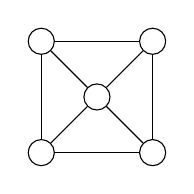
\begin{tikzpicture}[main/.style = {draw, circle}] 
            \node[main] (1) {};
            \node[main] (2) [above left of=1] {}; 
            \node[main] (3) [above right of=1] {};
            \node[main] (4) [below right of=1] {}; 
            \node[main] (5) [below left of=1] {};
            \draw (1) -- (2);
            \draw (1) -- (3);
            \draw (1) -- (4);
            \draw (1) -- (5);
            \draw (2) -- (3) -- (4) -- (5) -- (2);
        \end{tikzpicture}
    \end{center}
\end{ejemplo}

\begin{ndef}[Grafo bipartido completo]
    \textbf{Grafo bipartido completo} \textbf{K$_{r,s}$}. Determinado por dos grupos de vértices, con $r$ y $s$ vértices respectivamente. Los lados unen cada vértice de un grupo con todos los demás vértices del otro grupo.
\end{ndef}
\begin{ejemplo} $K_{2,2}$ y $K_{2,3}$ respectivamente:
    \begin{center}
        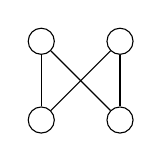
\begin{tikzpicture}[main/.style = {draw, circle}] 
            \node[main] (1) {}; 
            \node[main] (2) [right of=1] {}; 
            \node[main] (3) [below of=2] {};
            \node[main] (4) [left of=3] {};
            \draw (1) -- (4);
            \draw (1) -- (3);
            \draw (2) -- (3);
            \draw (2) -- (4);
        \end{tikzpicture}
        \quad\quad\quad\quad
        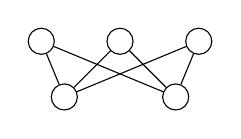
\begin{tikzpicture}[main/.style = {draw, circle}]
            \node[main] (3) {};
            \node[main] (1) [below left of=3] {};
            \node[main] (2) [below right of=3] {}; 
            \node[main] (4) [left of=3] {}; 
            \node[main] (5) [right of=3] {};
            \draw (1) -- (3);
            \draw (1) -- (4);
            \draw (1) -- (5);
            \draw (2) -- (3);
            \draw (2) -- (4);
            \draw (2) -- (5);
        \end{tikzpicture}
    \end{center}
\end{ejemplo}

\subsection{Sucesiones gráficas}
\begin{ndef}
    Sean $d_1,d_2,\cdots,d_n \in \nat$. Decimos que la sucesión $d_1,d_2,\cdots,d_n$ es una \textbf{sucesión gráfica} si existe un grafo $G$
    sin lazos ni lados paralelos, con conjunto de vértices $V = \{v_1,v_2,\cdots,v_n\}$ tal que $d_i = gr(v_i)$.
    Si $d_1,d_2,\cdots,d_n$ es una sucesión gráfica y $G$ es un grafo con $n$ vértices cuyos grados son los términos de la sucesión, diremos que $G$ es una \textbf{realización de la sucesión} $d_1,d_2,\cdots,d_n$.
\end{ndef}
\begin{obs}
    Dos condiciones necesarias para que una sucesión sea gráfica son que el la suma de los elementos de la sucesión sea par y que cualquier elemento de la sucesión debe ser menor que el número de elementos de ella.
\end{obs}

\begin{nth}[Havel-Hakimi]
    Sea $d_1,d_2,\cdots,d_n \in \nat$ una sucesión. Supongamos que están ordenados en orden decreciente, es decir, $d_1 \geq d_2 \geq \cdots \geq d_n$ y que $d_1 < n$.
    Entonces esta sucesión es gráfica si, y sólo si, lo es la sucesión $d_2 -1, \cdots, d_{d_1+1}-1, d_{d_1+2}-1, \cdots, d_n$.
\end{nth}

A la hora de aplicar este teorema, se suelen utilizar los siguientes algoritmos:

\subsubsection{Algoritmo de demolición}
Decide si una sucesión finita es una sucesión gráfica generando un número finito de sucesiones finitas.
\begin{enumerate}
    \item ¿Son todos los elementos de la sucesión 0? En caso afirmativo la sucesión es gráfica y hemos acabado.
    \item ¿Existe un número en la sucesión que es mayor o igual que el número de elementos no nulos de la sucesión? En caso afirmativo la sucesión no es gráfica y hemos acabado.
    \item Elige un vértice que cumpla que no hay ninguno en la sucesión con mayor grado y márcalo (pivote). Si elgrado marcado esr, elige r vértices que cumplan que entre los no elegidos no hay uno con mayor grado que alguno de los elegidos.
    \item Genera una nueva sucesión poniendo a cero el marcado (pivote) y disminuyendo en una unidad los elegidos.
    \item Vuelve a 1 con la nueva sucesión.
\end{enumerate}

\subsubsection{Algoritmo de reconstrucción paso a paso}
Si el algoritmo de demolición da como salida sucesión gráfica, se construye un grafo para cada fila del algoritmo de demolición leyendo las filas de abajo hacia arriba.
\begin{enumerate}
    \item Partimos del grafo nulo con n vértices que corresponde a la última fila de todos ceros.
    \item Pasamos de una fila a la superior añadiendo al grafo de la filarlados que conectan el vértice marcado en la fila superior con los elegidos (los que aumentan el grado en1).
\end{enumerate}

\subsection{Grafos de Euler}
\begin{ndef}
    Sea $G$ un grafo conexo. Un \textbf{camino de Euler} es un recorrido en el que aparecen todos los lados. Un \textbf{circuito de Euler} es un camino de Euler que es cerrado. Un \textbf{grafo de Euler} es un grafo con un circuito de Euler.
\end{ndef}

\begin{nprop}
    Sea $G$ un grafo. Entonces si $G$ tiene un circuito de Euler, el grado de cada vértice es par, mientras que si $G$ tiene un camino de Euler, $G$ tiene exactamente dos vértices de grado impar (que son donde empieza y donde acaba el camino).
\end{nprop}

\begin{nth}
    Sea $G$ un grafo conexo. Entonces $G$ es un grafo de Euler si, y sólo si, el grado de cada vértice es par.
\end{nth}

\begin{lema}
    Sea $G$ un grafo en el que cada vértice tiene grado mayor que 1. Entonces $G$ contiene un circuito (y por tanto un ciclo).
\end{lema}

\begin{ncor}
    Sea $G$ un grafo conexo. Entonces $G$ tiene un camino de Euler si, y sólo si, $G$ tiene exactamente dos vértices de grado impar.
\end{ncor}

\subsubsection{Algoritmo de Fleury}
Como entrada tenemos un grafo $G$ y como salida, dos sucesiones $S_V$ y $S_E$, siendo éstas las sucesiones de vértices y lados del camino buscado.
\begin{enumerate}
    \item Si todos los vértices son de grado par, elegimos un vértice cualquiera $v$. Si $G$ tiene dos vértices de grado impar, elegimos uno de estos vértices.
    \item Hacemos $S_V = v$ y $S_E = [\ ]$.
    \item Si $G$ tiene sólo a $v$, devuelve $S_V$ y $S_E$, y termina.
    \item Si hay un único lado $e$ que incida en $v$, llamamos $w$ al otro vértice donde incida el lado $e$; quitamos de $G$ el vértice $v$ y el lado $e$ y vamos al paso 6.
    \item Si hay más de un lado $e$ que incida en $v$, elegimos uno de estos de forma que al quitarlo el grafo $G$ siga siendo conexo. Llamamos $e$ a dicho lado y $w$ al otro vértice en el que incide $e$.
    \item Añadimos $w$ al final de $S_V$ y $e$ al final de $S_E$.
    \item Cambiamos $v$ por $w$ y volvemos al paso 3.
\end{enumerate}

\subsection{Grafos de Hamilton}
\begin{ndef}
    Sea $G$ un grafo. Un \textbf{camino de Hamilton} es un camino que recorre todos los vértices una sola vez.
\end{ndef}
Un \textbf{circuito de Hamilton} es un camino cerrado que recorre todos los vértices una sola vez (salvo los extremos). Un grafo con un circuito de Hamilton se denomina \textbf{grafo de Hamilton} o \textbf{grafo hamiltoniano}.
\begin{obs}
    Si hay un vértice de grado 1, entonces el grafo no es de Hamilton.
\end{obs}
\begin{nth}
    Sea $G$ un grafo con $n$ vértices. Entonces:
    \begin{enumerate}
        \item Si el número de lados es mayor o igual que $\frac{1}{2}(n-1)(n-2) + 2$ entonces el grafo es hamiltoniano.
        \item Si $n\geq 3$ y para cada par de vértices no adyacentes se verifica que $gr(v) +gr(w)\geq n$, entonces $G$ es un grafo de Hamilton.
    \end{enumerate}
\end{nth}

\subsection{Grafos bipartidos}
\begin{ndef}
    Sea $G= (V, E)$ un grafo. Se dice que $G$ es bipartido si podemos descomponer $V$ en dos subconjuntos disjuntos $V_1$ y $V_2$ de forma que todo lado incide en un vértice de $V_1$ y en un vértice de $V_2$. Un grafo $G= (V, E)$ se dice bipartido completo si es bipartido, y para cada $v_1 \in V_1$ y $v_2\ \in V_2$ existe un único lado $e \in E$ tal que $\gamma_G(e) =\{v1, v2\}$.
\end{ndef}
Un grafo bipartido completo está completamente determinado por el cardinal de $V_1$ y $V_2$. Si $G$ es un grafo bipartido completo en el que $V_1$ tiene cardinal $m$ y $V_2$ tiene cardinal $n$, entonces denotaremos a $G$ como $K_{m,n}$.
\begin{nth}
    Sea $G= (V, E)$ un grafo. Entonces $G$ es bipartido si, y sólo si, $G$ no contiene ciclos de longitud impar.
\end{nth}
\begin{lema}
    Sea $G$ un grafo bipartido con partición del conjunto de vértices $V = V_1 \cup V_2$. Supongamos qu $v_1v_2\cdots v_m$ es un camino en $G$ y que $v_1 \in V_1$. Entonces $\{v_1,v_3,v_5,\cdots\} \subseteq V_1$ y $\{v_2,v_4,\cdots\} \subseteq V_2$.
\end{lema}
\begin{nprop}
    Sea $G$ un grafo bipartido con partición $V_1$ y $V_2$. Supongamos que $|V_1|=n$ y $|V_2|=m$. Entonces:
    \begin{itemize}
        \item Si $G$ tiene un camino de Hamilton, entonces $|n-m| \leq 1$.
        \item Si $G$ es un grafo de Hamilton, entonces $n=m$.
        \item Si $G$ es completo y $|n-m|\leq 1$ entonces $G$ tiene un camino de Hamilton.
        \item Si $G$ es completo y $n=m$ entonces $G$ es un grafo de Hamilton.
    \end{itemize}
\end{nprop}

\subsection{Grafos planos}
\begin{ndef}
    Sea $G$ un grafo. Una representación de $G$ se dice plana si los vértices y los lados se encuentran todos en un plano, y las líneas que representan dos lados distintos no se cortan.
\end{ndef}
Un grafo se dice \textbf{plano} si admite una representación plana.

\begin{nth}[Característica de Euler]
    Sea $G$ un grafo plano y conexo. Llamemos $v$ al número de vértices, $l$ al número de lados y $c$ al número de caras de una representación plana. Entonces $v-l+c= 2$. En general, si $G$ es un grafo plano, y $\chi$ es el número de componentes conexas entonces $v-l+c= 1+\chi $.
\end{nth}
\begin{ncor}
    En un poliedro, si $v$ es el número de vértices; $l$ es el número de aristas y $c$ es el número de caras entonces $v-l+c= 2$.
\end{ncor}
\begin{ncor}
    Sea $G$ un grafo plano, conexo, sin lazos ni lados paralelos. Entonces $3c\leq 2e$ y $e \leq 3v-6$.
\end{ncor}
\begin{ndef}
    Sea $G$ un grafo. Una contracción simple de $G$ es el resultado de indentificar en $G$ dos vértices adyacentes.
\end{ndef}
\begin{nota}
    Una contracción de $G$ es una cadena de contracciones simples.
\end{nota}
\begin{nth}[Kuratowski]
    Sea $G$ un grafo. Entonces $G$ es plano si, y sólo si, ningún subgrafo suyo puede contraerse a $K_5$ ni a $K_{3,3}$.
\end{nth}

\subsection{Coloración de grafos}
\begin{ndef}
    Sea $G= (V, E)$ un grafo. Una \textbf{coloración} $G$ es una aplicación $f:V\to C$, donde $C$ es un conjunto, de tal forma que para cualquier $e\in E$, si $\gamma_G(e) =\{v, w\}$ con $v \neq w$ entonces $f(u)\neq f(v)$.
\end{ndef}
\begin{ndef}
    Sea $G$ un grafo y $x\in\nat$. Vamos a denotar por $p(G, x)$ al número de coloraciones distintas, con $n$ colores, que tiene el grafo $G$.
\end{ndef}
A partir de aquí denotaremos las \textbf{potencias descendentes} $p(K_n,x) = x^{\underline{n}} = x(x-1)\cdots(x-n+1)$.

\subsubsection{Algoritmo de la suma}
La fórmula $p(G_e,x)=p(G,x) + p(G'_e,x)$ nos indica que dado un grafo simple $G_e$ hallar su polinomio cromático se reduce a sumar los polinomios cromáticos de los grafos $G$ y $G'_e$. $G$ tiene un lado más que $G_e$ (lado que une dos vértices no adyacentes de $G_e$) y $G'_e$ tiene un vértice menos que $G_e$. En un número finito de pasos todos los grafos obtenidos serán completos que es la condición de parada.

\subsubsection{Algoritmo de la resta}
La fórmula anterior podemos escribirla como $p(G,x)=p(G_e,x) - p(G'_e,x)$ que nos permite reducir el cálculo del polinomio cromático de un grafo al cálculo de polinomios cromáticos de grafos más pequeños (con menos lados o con menos vértices). La condición de parada es ambigua. Paramos cuando obtengamos grafos de los que conozcamos sus polinomios cromáticos.

\begin{ejemplo}
    e
\end{ejemplo}

\subsection{Árboles}
Los árboles son un tipo especial de grafos estudiados por primera vez por Kirchhoff en 1847 en su trabajo de redes eléctricas y actualmente es una de las estructuras más utilizadas en distintas disciplinas.
\begin{ndef}[Árbol]
    Un \textbf{árbol} es un grafo conexo y acíclico.
\end{ndef}
\begin{ndef}[Bosque]
    Un \textbf{bosque} es un grafo acíclico.
\end{ndef}
\begin{ejemplo} En el siguiente ejemplo, tenemos tres árboles que en su conjunto conforman un bosque:
    \begin{center}
    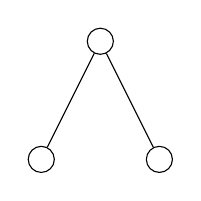
\begin{tikzpicture}[nodes={draw, circle}, -]
        \node {}
        child {node {}}
        child {node {}};
    \end{tikzpicture}
    \quad\quad\quad
    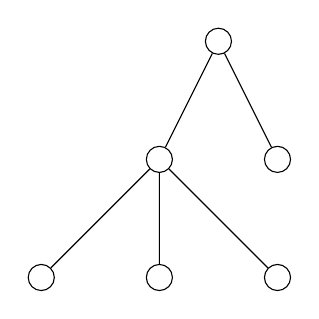
\begin{tikzpicture}[nodes={draw, circle}, -]
        \node{}
    child { node {} 
        child { node {} }
        child { node {} }
        child { node {} }
    }
    child { node {} };
    \end{tikzpicture}
    \quad\quad\quad
    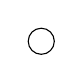
\begin{tikzpicture}[nodes={draw, circle}, -]
        \node {};
    \end{tikzpicture}
    \end{center}
\end{ejemplo}


\begin{nth}
    Todo árbol es un grafo plano.
\end{nth}
\begin{ncor}
    Sea $G$ un grafo conexo con $n$ vértices. Entonces $G$ es un árbol si, y sólo si, $G$ tiene $n-1$ lados.
\end{ncor}
\begin{nth}
    Sea $G$ un grafo con $n$ vértices, sin lados paralelos ni lazos. Entonces son equivalentes:
    \begin{enumerate}
        \item $G$ es un árbol.
        \item $G$ es acíclico y tiene $n-1$ lados.
        \item $G$ es conexo y tiene $n-1$ lados.
        \item $G$ es conexo, pero si le quitamos un lado deja de serlo, es decir, todos los lados son puentes.
        \item $G$ Dos vértices cualesquiera están unidos por un único camino simple.
        \item $G$ no tiene ciclos, pero si le añadimos un lado aparece un sólo ciclo.
    \end{enumerate}
\end{nth}
\begin{ncor}
    Si $G$ es un bosque con $n$ vértices y $k$ componentes, entonces $G$ tiene $n-k$ lados.
\end{ncor}

\subsubsection{Árboles generadores}
\begin{ndef}
    Un \textbf{árbol generador} (de expansión, abarcador) de un grafo conexo es un subgrafo que tiene todos los vértices del grafo y es un árbol.
\end{ndef}
\begin{lema}
    SeaGun grafo conexo que contiene un ciclo. Entonces, si quitamos uno de los lados del ciclo el grafosigue siendo conexo.
\end{lema}
\begin{nprop}
    Todo grafo conexo tiene un árbol generador.
\end{nprop}

\subsubsection{Estrategias de obtención de árboles generadores}
\textbf{\underline{Obtención de árboles generadores no ponderados}} \\

Dado un grafo conexo con $n$ vértices y $l$ lados hay dos estrategias para obtener un árbol generador:
\begin{itemize}
\item\textbf{Building-up (constructiva):} \\
Se eligen $n-1$ lados de uno en uno de forma que cada uno no forme ciclos con los anteriormente elegidos.
\item\textbf{Cutting-down (destructiva):} \\
Se descartan $l-(n-1) =l-n+ 1$ lados de uno en uno de forma que cada uno de los que se descartan rompa un ciclo (forme parte de un ciclo) del grafo que va quedando.
\end{itemize}
\textbf{\underline{Obtención de árboles generadores de peso mínimo}} \\

Se utilizan para dado un grafo ponderado conexo encontrar un árbol generador de peso mínimo:
\begin{itemize}
    \item\textbf{Algoritmo de Kruskal (constructivo):} \\
    Aplicación de la estrategia building-up a una sucesión de aristas de pesos no decrecientes.
    \item\textbf{Algoritmo de Kruskal (destructivo):} \\
    Aplicación de la estrategia cutting-down a una sucesión de aristas de pesos no crecientes.
    \item\textbf{Algoritmo de Prim:} \\
    Se trabaja con vértices y lados. Se parte de un vértice arbitrario $v$ que pasa al conjunto de los elegidos $T = \{v\}$ t $E=\{\}$. En cada paso, se añade un vértice $u$ a $T$ y un lado $e$ a $E$ con las condiciones:
    \begin{enumerate}
        \item que $u$ sea un vértice que no esté en $T$.
        \item  que $u$ sea adyacente mediante el lado $e$ a uno de $T$.
        \item que el lado $e$ no forme ciclo con los lados de $E$.
        \item que $e$ sea de peso mínimo entre los que cumplen las condiciones anteriores.
    \end{enumerate}
    Este proceso acaba cuando se han elegido $n-1$ lados.
\end{itemize}

\subsubsection{Árboles con raíz}
A continuación vamos a definir una serie de conceptos acerca de los árboles con raíz:
\begin{ndef}[Árbol con raíz]
    Un árbol en el que se elige un vértice es un árbol con raíz.
\end{ndef}
\begin{ndef}[Raíz]
    El vértice elegido se llama raíz.
\end{ndef}
\begin{ndef}[Nodo]
    Los vértices de un árbol con raíz se llaman nodos.
\end{ndef}
\begin{ndef}[Nivel]
    El nivel o profundidad de un nodo es la longitud del único camino simple que existe de la raíz al nodo.
\end{ndef}
\begin{ndef}[Hijo]
    Se llaman hijos de un nodo a los nodos adyacentes con mayor nivel.
\end{ndef}
\begin{ndef}[Descendiente]
    Los descendientes de un nodo son sus hijos y los descendientes de sus hijos.
\end{ndef}
\begin{ejemplo} En el siguiente árbol con raíz:
    \begin{center}
        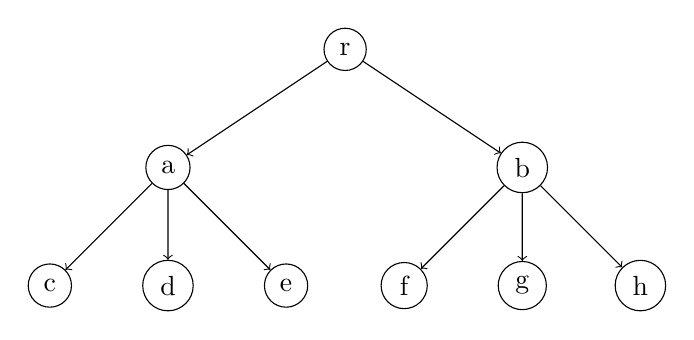
\begin{tikzpicture}[nodes={draw, circle}, ->]
            \node{r}
            child { node {a} 
                child { node {c} }
                child { node {d} }
                child { node {e} }
            }
            child [missing]
            child [missing]
            child {node {b} 
                child { node {f} }
                child { node {g} }
                child { node {h} }
            };
            \end{tikzpicture}
    \end{center}
    La raíz es $r$; $a$ tiene nivel 1; $h$ tiene nivel 2; los hijos de $b$ son $f$, $g$ y $h$; $r$ es padre de $a$ y $b$, y todos los nodos son descendientes de $r$ menos él mismo.
\end{ejemplo}

\begin{ndef}[Hoja]
    Una hoja es un nodo sin descendientes.
\end{ndef}
\begin{ndef}[Altura de un árbol]
    La altura de un árbol es el mayor de los niveles de sus nodos.
\end{ndef}
\begin{ndef}[Subárbol con raíz]
    El subárbol con raíz un nodo es el subárbol formado por el nodo y sus descendientes.
\end{ndef}
\begin{ndef}[Altura de un nodo]
    La altura de un nodo es la altura del subárbol que lo tiene como raíz.
\end{ndef}
\begin{ndef}[Rango de un nodo]
    El rango de un nodo es una cualidad del nodo que sirve para compararlo con los que tienen el mismo nivel. Un nodo tiene rango menor que otro si está a su izquierda.
\end{ndef}

\begin{ejemplo} En el árbol del ejemplo anterior, las hojas eran $c,d,e,f,g$ y $h$. La altura del árbol es 2. El subárbol con raíz $a$ es:
    \begin{center}
        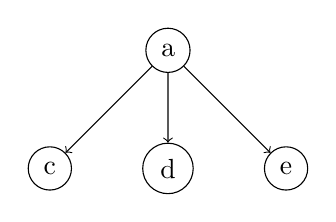
\begin{tikzpicture}[nodes={draw, circle}, ->]
            \node{a}
            child { node {c} }
            child { node {d} }
            child { node {e} };
        \end{tikzpicture}
    \end{center}
\end{ejemplo}

\subsubsection{Recorrido de árboles con raíz}
A la hora de recorrer un árbol podemos hacerlo en función de su nivel o profundidad, su altura o su rango. Estos son los recorridos que estudiaremos:
\begin{itemize}
    \item\textbf{Recorrido en Preorden:} 
    Primero se recorre la raíz y después se recorren los subárboles hijos en preorder en orden creciente del rango de sus raíces.
    \item\textbf{Recorrido en Postorden:} 
    Primero se recorren los subárboles hijos en postorder en orden creciente del rango de sus raíces y después se recorre la raíz.
    \item\textbf{Recorrido en Inorden.} 
    Primero se recorre el subárbol hijo de menor rango en inorder después la raíz y por último se recorren en inorder el resto de subárboles hijos en orden creciente del rango de sus raíces. Algunos autores sólo consideran este recorrido para árboles binarios.
    \item\textbf{Recorrido Top-Down:} 
    Se recorren los nodos en orden creciente de profundidad o nivel y dentro de un nivel en orden creciente de rangos. Es el recorrido en anchura usual y es trivial en el sentido de que es el orden de lectura de izquierda a derecha y de arriba hacia abajo.
    \item\textbf{Recorrido Bottom-up:} 
    Es el más complejo y difícil. Se recorren los nodos en orden creciente de altura, dentro de los de misma altura en orden creciente de profundidad y dentro de los de la misma altura y profundidad en orden creciente de rango.
\end{itemize}
\begin{ejemplo}
    A partir del anterior ejemplo, los recorridos serían:
    \begin{itemize}
        \item\textbf{Preorden:} $r,a,c,d,e,b,f,g,h$.
        \item\textbf{Postorden:} $c,d,e,a,f,g,h,b,r$.
        \item\textbf{Inorden:} $c,a,d,e,r,f,b,g,h$.
        \item\textbf{Top-Down:} $r,a,b,c,d,e,f,g,h$.
        \item\textbf{Bottom-up:} $c,d,e,f,g,h,a,b,r$.
    \end{itemize}
\end{ejemplo}

\subsubsection{Árboles etiquetados}
\begin{ndef}[Árbol etiquetado]
    Un árbol etiquetado es un árbol connvértices en que los vértices tienen como etiquetas los números naturales $\{1,2,\cdots,n\}$.
\end{ndef}
\begin{ndef}[Isomorfismo]
    Dos árboles etiquetados son isomorfos si tienen el mismo número de vértices y la aplicación identidad es un isomorfismo de grafos.
\end{ndef}
\begin{nth}
    El número de árboles etiquetados con $n$ vértices es $n^{n-2}$.
\end{nth}

\subsubsection{Códigos de Prüfer}
Suponemos los árboles etiquetados con los números naturales de $1$ a $n$. Llamamos \textbf{código de Prüfer} de un árbol etiquetado a la sucesión de longitud $n-2$ obtenida de la siguiente forma:
\begin{enumerate}
    \item Se parte de la sucesión vacía (código vacío) y del árbol etiquetado $T$.
    \item Si $T$ tiene dos vértices se devuelve el código y fin.
    \item Se determina la hoja con menor etiqueta del árbol $T$ se añade al código la etiqueta del adyacente a la hoja seleccionada y $T$ pasa a ser el árbol con la hoja seleccionada suprimida.
    \item Vuelve a $2$ con el nuevo código y el nuevo árbol.
\end{enumerate}
\textbf{Generación de un árbol etiquetado con un código dado:}
\begin{enumerate}
    \item Se parte del código $c$ de longitud $n-2$, del conjunto $V=\{1,2,\cdots,n\}$ y $T$ el grafo vacío con $n$ vértices etiquetado.
    \item Si $c$ es vacío y $V$ tiene dos vértices se pone un lado entre los vértices de $V$, se devuelve $T$ y se acaba.
    \item Se determina el menor número de $V$ que no está en $c$ se añade a $T$ un lado entre ese menor número y el primer elemento del código. Se quita de $V$ el elemento seleccionado y de $c$ su primer elemento.
    \item Vuelve a $2$ con el nuevo código, el nuevo conjunto $V$ y el nuevo grafo $T$.
\end{enumerate}
\begin{ejemplo}
    Vamos a hallar el árbol con código de Prüfer (6,4,3,3). Tiene 6 vértices y 5 lados. Aplicando el álgoritmo los lados son 6-1, 4-2, 3-4, 3-5 y 3-6, resultando
    \begin{center}
        \begin{tikzpicture}[new set=import nodes]
            \begin{scope}[nodes={set=import nodes}] % make all nodes part of this set
            \node [black] (5) at (2,1) {$5$};
            \end{scope}
            \graph {
            (import nodes);
            % "import" the nodes
            1 -- 6 -- 3 -- 5 -- 3 -- 4 -- 2;
            };

        \end{tikzpicture}
    \end{center}
\end{ejemplo}


\newpage
\section{Lógica proposicional}
\subsection{Lenguaje proposicional}
La \textbf{lógica proposicional}, también llamada lógica de enunciados o de orden cero, es un sistema formal cuyos elementos más simples representan proposiciones o enunciados, y cuyas constantes lógicas, llamadas conexiones lógicas, representan operaciones sobre proposiciones, capaces de formar otras proposiciones de mayor complejidad.

\subsubsection{Conexiones lógicas}
Las \textbf{conexiones lógicas}, también conocidas como conectivas o constantes lógicas, son símbolos o palabras que se utilizan para conectar dos \textbf{enunciados, proposiciones o sentencias} (atómicas o moleculares), de modo que el valor de verdad de la fórmula compuesta depende del valor de verdad de las fórmulas componentes.
Diremos que una sentencia es \textbf{atómica} cuando los enunciados del lenguaje no se puedan dividir en otros.
\begin{nota}
    Usaremos las primeras letras minúsculas del alfabeto griego para simbolizar los enunciados atómicos y las letras minúsculas a partir de la $p$ para representar los enunciados de lo que nos interesa conocer el significado.
\end{nota}

Para dos enunciados $\alpha,\ \beta$, las partículas conectivas que emplearemos son:
\begin{itemize}
    \item \textbf{Negación} ($\neg \alpha$): el \textit{no} se antepone a un enunciado y da lugar a otro enunciado.
          \begin{center}
              \begin{tabular}{ |c|c|  }
                  \hline
                  $\alpha$ & $\neg \alpha$ \\
                  \hline
                  0        & 1             \\
                  1        & 0             \\
                  \hline
              \end{tabular}
          \end{center}

    \item \textbf{Conjunción} ($\alpha \wedge \beta$): la \textit{y} se corresponde con su sentido más usual en el lenguaje natural.
          \begin{center}
              \begin{tabular}{ |c|c|c|  }
                  \hline
                  $\alpha$ & $\beta$ & $\alpha \wedge \beta$ \\
                  \hline
                  0        & 0       & 0                     \\
                  0        & 1       & 0                     \\
                  1        & 0       & 0                     \\
                  1        & 1       & 1                     \\
                  \hline
              \end{tabular}
          \end{center}

    \item \textbf{Disyunción} ($\alpha \vee \beta$): la \textit{o} se corresponde con uno de los dos sentidos más usuales en el lenguaje natural.
          \begin{center}
              \begin{tabular}{ |c|c|c|  }
                  \hline
                  $\alpha$ & $\beta$ & $\alpha \vee \beta$ \\
                  \hline
                  0        & 0       & 0                   \\
                  0        & 1       & 1                   \\
                  1        & 0       & 1                   \\
                  1        & 1       & 1                   \\
                  \hline
              \end{tabular}
          \end{center}

    \item \textbf{Implicación} ($\alpha \rightarrow \beta$): el \textit{cuando} puede emplearse en sentido condicional como el \textit{si...entonces...} y otras veces en sentido temporal.
          \begin{center}
              \begin{tabular}{ |c|c|c|  }
                  \hline
                  $\alpha$ & $\beta$ & $\alpha \rightarrow \beta$ \\
                  \hline
                  0        & 0       & 1                          \\
                  0        & 1       & 1                          \\
                  1        & 0       & 0                          \\
                  1        & 1       & 1                          \\
                  \hline
              \end{tabular}
          \end{center}

    \item \textbf{Doble implicación} ($\alpha \leftrightarrow \beta$): el \textit{si, y solo si,} sucede cuando se cumple $\alpha \rightarrow \beta$ y $\beta \rightarrow \alpha$.
          \begin{center}
              \begin{tabular}{ |c|c|c|  }
                  \hline
                  $\alpha$ & $\beta$ & $\alpha \leftrightarrow \beta$ \\
                  \hline
                  0        & 0       & 1                              \\
                  0        & 1       & 0                              \\
                  1        & 0       & 0                              \\
                  1        & 1       & 1                              \\
                  \hline
              \end{tabular}
          \end{center}
\end{itemize}

\subsubsection{Elementos del lenguaje proposicional}
Como hemos dicho anteriormente, los elementos de la lógica proposicional son los enunciados. Para desgranarlos y comprenderlos, usaremos la estructura en árbol.
Así, una fórmula sería un árbol queen las hojas tiene las fórmulas atómicas que intervienen y en el resto de los nodos las conectivas.
\begin{ejemplo}
    e
\end{ejemplo}

\subsection{Semántica de la lógica proposicional}
\subsubsection{Interpretaciones}
\begin{ndef}[Interpretación]
    Dado un lenguaje proposicional construido sobre el conjunto $X$, una \textbf{valoración, interpretación o mundo posible}, es una aplicación $v: X \rightarrow \mathbb{Z}_2$.
\end{ndef}
Dicha aplicación asigna un valor de la verdad a cada proposición atómica.
Para una valoración $v$ y una fórmula atómica $a$, para $v(a)=0$ diremos que $v$ es \textbf{falsa} en el mundo $v$ y para $v(a)=1$ diremos que $v$ es \textbf{verdadera} en el mundo $v$.

Una forma muy útil de expresar el valor de la verdad de una proposición es a través de su \textbf{polinomio de Gegalkine}. Éste es el anillo de polinomios sobre $\mathbb{Z}_2$. Para obtenerlo (aunque formalmente sea incorrecto), sustituiremos las siguientes expresiones proposicionales por su equivalente en el polinomio:
\begin{align*}
    \alpha \lor \beta = v(\alpha) + v(\beta) + v(\alpha) \cdot v(\beta) \\
    \alpha \land \beta = v(\alpha) \cdot v(\beta)                       \\
    \alpha \rightarrow \beta = 1 + v(\alpha) + v(\alpha) \cdot v(\beta) \\
    \alpha \leftrightarrow \beta = 1 + v(\alpha) + v(\beta)             \\
    \neg \alpha = 1 + v(\alpha)
\end{align*}

Otra forma de expresar una fórmula proposicional es mediante su \textbf{tabla de la verdad}. Para ella, podemos crear una tabla con $2^n$ mundos posibles.

\begin{ejemplo}
    Para la fórmula $\alpha = \neg (a \rightarrow b) \rightarrow (\neg a \rightarrow \neg b)$, hagámoslo por partes:
    \begin{center}
        $\neg (a \rightarrow b) = 1 + a \rightarrow b = 1 + 1 + a + ab = a + ab$ \\
        $\neg a \rightarrow \neg b = 1 + \neg a + (\neg a)(\neg b) = 1 + 1 + a + (1 + a)(1 + b) = a +1 +a +b +ab = 1 + b + ab$ \\
        $\alpha = 1 + \neg (a \rightarrow b) + \neg (a \rightarrow b) (\neg a \rightarrow \neg b) = 1 +a+ab+ (a+ab)(1 +b+ab) = 1 +a+ab+a+ab+ab+ab+ab+ab = 1$
    \end{center}

    Por otro lado, su tabla de la verdad sería:
    \begin{center}
        \begin{tabular}{|c|c||c|c|c|c|c|c|}
            \hline
            $a$ & $b$ & $a \rightarrow b$ & $\neg(a \rightarrow b)$ & $\neg a$ & $\neg b$ & $\neg a \rightarrow \neg b$ & $\neg (a \rightarrow b) \rightarrow (\neg a \rightarrow \neg b)$ \\
            \hline
            0   & 0   & 1                 & 0                       & 1        & 1        & 1                           & 1                                                                \\
            0   & 1   & 1                 & 0                       & 1        & 0        & 0                           & 1                                                                \\
            1   & 0   & 0                 & 1                       & 0        & 1        & 1                           & 1                                                                \\
            1   & 1   & 1                 & 0                       & 0        & 0        & 1                           & 1                                                                \\
            \hline
        \end{tabular}
    \end{center}
    Vemos que en ambos casos la solución es constantemente igual a 1.
\end{ejemplo}

A las fórmulas cuyo valor de la verdad sea constantemente 1 las llamaremos \textbf{tautologías}. Si la fórmula es cierta en, al menos, algún mundo posible, diremos que es \textbf{satisfacible}.
Por otro lado, las que son constantemente igual a 0 las llamaremos \textbf{contradicciones}.
\begin{nota}
    El uso de la palabra tautología de dicha clasificación de fórmulas fue usada por primera vez por \textbf{Ludwig Josef Johann Wittgenstein}.
\end{nota}

Cuando trabajemos con fórmulas lógicas, es conveniente conocer ciertas tautologías y equivalencias lógicas que nos ayudarán a identificar fórmulas con mayor facilidad.

\subsection{Consecuencia lógica}
\subsubsection{Conjuntos satisfacibles e insatisfacibles}
\begin{ndef}
    Sea $\Gamma = \{\gamma_1, \gamma_2, \cdots, \gamma_n\}$ un conjunto de fórmulas de un lenguaje proposicional. Se dice que $\Gamma$ es \textbf{satisfacible} si existe un mundo en que todas son verdaderas.
    Es decir, existe $v$ tal que $v(\gamma_1) = v(\gamma_2) = \cdots = v(\gamma_n) = 1$.
\end{ndef}
\begin{nota}
    Si $\Gamma = \emptyset$, entonces $\Gamma$ es satisfacible.
\end{nota}
Cuando un conjunto de fórmulas no sea satisfacible, diremos que es \textbf{insatisfacible}.

\begin{nth}
    Sea $\Gamma = \{\gamma_1, \gamma_2, \cdots, \gamma_n\}$ un conjunto de fórmulas. Entonces son equivalentes:
    \begin{enumerate}
        \item $\Gamma$ es insatisfacible.
        \item $\gamma_1 \land \gamma_2 \land \cdots \land \gamma_n$ es contradicción.
        \item Para cualquier valoración $v$, $\prod^n_{i=1} v(\gamma_i) = 0$.
    \end{enumerate}
\end{nth}
\begin{ejemplo}
    e
\end{ejemplo}

\subsubsection{Implicación semántica}
\begin{ndef}
    Dado un conjunto de fórmulas $\Gamma$ —posiblemente vacío— y una fórmula $\varphi$ decimos que $\Gamma$ \textbf{implica semánticamente a $\varphi$}, abreviadamente $\Gamma \models \varphi$, si para toda valoración $v$ se tiene $v(\varphi) = 1$ siempre que para toda fórmula $\gamma$ de $\Gamma$ valga $v(\gamma) = 1$.
    Si $\Gamma$ consta solamente de las fórmulas $\gamma_1, \gamma_2, \cdots, \gamma_n$, en lugar de$\{\gamma_1, \gamma_2, \cdots, \gamma_n\} \models \varphi$ escribimos $\gamma_1, \gamma_2, \cdots, \gamma_n \models \varphi$ y cuando $\Gamma = \emptyset$ escribimos simplemente $\models \varphi$ en lugar de $\emptyset \models \varphi$.
\end{ndef}
\begin{ejemplo}
    e
\end{ejemplo}

\subsubsection{Teorema de la deducción}
Ahora presentaremos un \textbf{metateorema} (teorema acerca de teoremas formales y deducciones formales), que expresa simbólicamente una forma de razonamiento que frecuentemente empleamos cuando discurrimos informalmente en matemáticas.
\begin{nth}[de la Deducción]
    Sea $\Gamma$ un conjunto de fórmulas (que podría ser vacío) de un lenguaje proposicional, y $\alpha,\beta$, otras dos fórmulas. Entonces las siguientes afirmaciones son equivalentes:
    \begin{enumerate}
        \item $\Gamma \models \alpha \to \beta$
        \item $\Gamma \cup \{\alpha\} \models \beta$
    \end{enumerate}
\end{nth}
\begin{nota}
    Este teorema se menciona para poder realizar los ejercicios. Sin embargo, no vamos a profundizar mucho en él.
\end{nota}

\begin{ejemplo}
    e
\end{ejemplo}

\subsection{Forma clausulada de una fórmula}
\begin{ndef}
    Una fórmula se dice que está en \textbf{forma clausulada} si está escrita como conjunción de cláusulas.
\end{ndef}

\begin{nth}
    Sea $\alpha$ una fórmula que no es tautología. Entonces existe otra fórmula $\beta$, lógicamente equivalente a $\alpha$ y que está en forma clausulada.
\end{nth}
\subsubsection{Algoritmo de la forma clausulada}
Vamos a dar un método para transformar una proposición $\delta$ en otra que sea lógicamente equivalente y que esté en forma clausulada. Para esto, podemos seguir los siguientes pasos:
\begin{enumerate}
    \item Eliminación del bicondicional. Si tenemos una subfórmula de la forma $\alpha_1 \leftrightarrow \alpha_2$, la sustituimos por $(\alpha_1 \rightarrow \alpha_2) \land (\alpha_2 \rightarrow \alpha_1)$.
    \item Eliminación del condicional. Si tenemos una subfórmula de la forma$\alpha_1 \rightarrow \alpha_2$ la sustituimos por $\neg\alpha_1 \lor \alpha_2$.
    \item Interiorización de la negación. Cualquier subfórmula de la forma:
          \begin{itemize}
              \item $\neg\neg \alpha$ la sustituimos por $\alpha$.
              \item $\neg (\alpha_1 \lor \alpha_2)$ la sustituimos por $\neg\alpha_1 \land \neg\alpha_2$.
              \item $\neg (\alpha_1 \land \alpha_2)$ la sustituimos por $\neg\alpha_1 \lor \neg\alpha_2$.
          \end{itemize}
          Llegados aquí, nos encontraremos una proposición en la que sólo intervienen las conectivas $\lor$,$\land$ y $\neg$. Además,esta última solo actua sobre las fórmulas atómicas.
    \item Distribución de la $\lor$ sobre la $\land$.Si tenemos una subfórmula de la forma $\alpha_1 \lor (\beta_1 \land \beta_2)$ la sustituimos por $(\alpha_1 \lor \beta_1) \land (\alpha_1 \lor \beta_2)$. Y lo mismo, si la subfórmula es de la forma $(\alpha1 \lor \alpha_2) \land \beta_1$ la sustituimos por $(\alpha_1 \lor \beta_1) \land (\alpha_2 \lor \beta_1)$.
    \item Eliminación de redundancias. Dentro de una cláusula eliminación de literales por idempotencia. Absorción de cláusulas más grandes por las mas chicas.
\end{enumerate}
\begin{ejemplo}
    e
\end{ejemplo}

\subsection{El problema de la implicación semántica}
Ahora vamos a estudiar si un conjunto de fórmulas es satisfacible o no.
\begin{nth}
    Sea $\Gamma$ un conjunto de fórmulas; $\Gamma'$ un conjunto de fórmulas que se obtiene sustituyendo cada fórmula de $\Gamma$ por una forma clausular de esa fórmula, y $\Gamma''$ el conjunto que resulta de sustituir cada fórmula de $\Gamma'$ por las cláusulas que la forman. Entonces son equivalentes:
    \begin{enumerate}
        \item $\Gamma$ es instisfacible.
        \item $\Gamma'$ es instisfacible.
        \item $\Gamma''$ es instisfacible.
    \end{enumerate}
\end{nth}

\subsubsection{Algoritmo de Davis-Putnam}
\begin{enumerate}
    \item Sea $\Sigma$ un conjunto de cláusulas. Supongamos que en $\Sigma$ hay una \textbf{cláusula unit} $\lambda$. Entonces $\Sigma$ es insatisfacible si, y sólo si, $\Sigma_\lambda$ es insatisfacible.
    \item Sea $\Sigma$ un conjunto de cláusulas. Supongamos que en $\Sigma$ aparece un \textbf{literal puro} $\lambda$. Es decir, hay al menos una cláusula en la que aparece el literal $\lambda$ y el literal $\lambda^c$ no aparece en ninguna. Entonces $\Sigma$ es insatisfacible si, y sólo si, $\Sigma_\lambda$ es insatisfacible.
    \item Sea $\Sigma$ un conjunto de cláusulas, y sea $\lambda$ un literal que aparece en alguna cláusula de $\Sigma$. Entonces: $\Sigma$ es insatisfacible si, y sólo si, $\Sigma_\lambda$ y $\Sigma_{\lambda^c}$ son insatisfacibles.
\end{enumerate}
\begin{ejemplo}
    e
\end{ejemplo}

\subsubsection{Método de resolución}
\begin{nth}
    Sean $\alpha,\beta,\gamma$ tres fórmulas en un lenguaje proposicional. Entonces $\{\alpha \lor \beta, \neg \alpha \lor \gamma\} \models \beta \lor \gamma$.
\end{nth}
Para poder aplicar dicho método, definamos previamente el concepto de resolvente. Para ello, denotaremos $C - \lambda$ a la cláusula resultante de eliminar el literal $\lambda$ de la cláusula $C$. Dicho esto:
\begin{ndef}
    Sean $C_1$ y $C_2$ dos cláusulas. Supongamos que $\lambda$ es un literal tal que aparece en la cláusula $C_1$ y $\lambda^c$ aparece en $C_2$. Una cláusula que sea equivalente a $(C_1 - \lambda) \lor (C_2 - \lambda^c)$ es lo que se denomina una \textbf{resolvente} de $C_1$ y $C_2$.
\end{ndef}
\begin{obs} En la definición de resolvente debemos tener en cuenta 2 casos especiales:
    \begin{enumerate}
        \item Si $(C_1-\lambda)\lor(C_2-\lambda)$ es una tautología, consideraremos $(C_1-\lambda)\lor(C_2-\lambda)$ una resolvente.
        \item Si $C_1=\lambda$ y $C_2=\lambda^c$, entonces la resolvente es $\square$.
    \end{enumerate}
\end{obs}
\begin{ndef}
    Sea $\Gamma$ un conjunto de cláusulas, y $C$ una cláusula. Una \textbf{deducción} (por resolución) de $C$ a partir de $\Gamma$ es una sucesión de cláusulas $C_1,C_2,\cdots,C_n$ donde:
    \begin{itemize}
        \item $C_n = C$.
        \item $C_i \in \Gamma$ o $C_i$ es una resolvente de dos cláusulas del conjunto $\{C_1,\cdots,C_{i-1}\}$.
    \end{itemize}
\end{ndef}
\begin{nth}[Principio de resolución]
    Sea $\Gamma$ un conjunto de cláusulas. Entonces $\Gamma$ es insatisfacible si, y sólo si, hay una deducción por resolución de la cláusula vacía.
\end{nth}
\begin{ejemplo}
    e
\end{ejemplo}
A partir del anterior teorema, podemos saber si un conjunto es insatisfacible. No obstante, podría darse que no podamos deducir la cláusula vacía. En ese caso, usaremos varias estrategias para calcular resolventes:

\subsubsection{Estrategias de resolución}
\underline{\textbf{Estrategia de saturación}}
\begin{enumerate}
    \item Esto, en realidad no es una estrategia. Se trata de calcular resolventes. Paramos, bien cuando encontremos la cláusula vacía, bien cuando no se puedan calcular más resolventes.
    \item Puesto que el número posible de cláusulas para un conjunto de $n$ fórmulas atómicas es $3^n$, este método siempre acaba, pero puede ser muy largo.
    \item Para seguir un cierto orden, partimos de nuestro conjunto de cláusulas, que llamaremos$\Sigma_0$.
    \item En una primera etapa calculamos todas las resolventes que podemos hacer con estas cláusulas, y las añadimos al conjunto. Tenemos así un nuevo conjunto $\Sigma_1$.
    \item En la siguiente etapa calculamos todas las resolventes que podemos hacer con las cláusulas de $\Sigma_1$. Al nuevo conjunto lo llamamos $\Sigma_2$.
    \item De esta forma, vamos obteniendo una sucesión de conjuntos de cláusulas $\Sigma_0 \subseteq \Sigma_1 \subseteq \Sigma_2 \subseteq \cdots$ que en algún momento tiene que estabilizarse. Si llegamos a ese momento sin haber obtenido la cláusula vacía el conjunto $\Sigma$ es satisfacible.
\end{enumerate}

\begin{ejemplo}
    e
\end{ejemplo}

\underline{\textbf{Resolución Lineal}} \\

Una deducción por resolución de una cláusula es \textbf{lineal} si es una sucesión de pasos de resolución que cumple que en cada paso de resolución que no sea el primero se utiliza la resolvente del paso anterior. Esto da lugar a un árbol con una estructura muy peculiar. \\
En los ejemplos que hemos hecho de resolución observamos que en todos ellos (salvo el segundo de los ejemplos 4.20) cada resolvente que hemos obtenido (a excepción de la primera) provenía de hacer una resolvente con una cláusula obtenida en el paso inmediatamente anterior junto con otra cláusula. Esto daba lugar a que en la representación que hacíamos de las resolventes, todas aparecieran formando una línea.

\begin{ejemplo}
    e
\end{ejemplo}

\underline{\textbf{Estrategias input}} \\

Dado un conjunto de cláusulas $\Sigma$, una deducción a partir de $\Sigma$ (por resolución) es \textbf{input} si al menos una de lasdos cláusulas que se usan para calcular cada una de las resolventes pertenece al conjunto $\Sigma$.

\begin{ejemplo}
    e
\end{ejemplo}

\begin{ndef}
    Dado un lenguaje proposicional construido sobre el conjunto $X$:
    \begin{enumerate}
        \item Un literal es \textbf{positivo} si es una fórmula atómica (es decir, si pertenece a $X$).
        \item Un literal es \textbf{negativo} si es el negado de una fórmula atómica.
        \item Una cláusula es \textbf{negativa} si todos los literales que aparecen en ella son literales negativos.
        \item Una cláusula es cláusula de \textbf{Horn} si tiene exactamente un literal positivo.
        \item Un conjunto de cláusulas es un \textbf{conjunto de Horn} si tiene exactamente una cláusula negativa, y el resto de las cláusulas son cláusulas de Horn.
    \end{enumerate}
\end{ndef}

\begin{nth}
    Sea $\Sigma$ un conjunto de cláusulas de un lenguaje proposicional que es un conjunto de Horn. Entonces $\Sigma$ es insatisfacible si, y sólo si, existe una deducción lineal-input de la cláusula vacía que se inicia en la cláusula negativa.
\end{nth}
\begin{obs} Del teorema anterior extraemos que:
    \begin{enumerate}
        \item \textbf{Un conjunto formado por cláusulas de Horn no es un conjunto de Horn}. En el primero no hay cláusulas negativas y es satisfacible mientras que en el segundo hay una.
        \item \textbf{Los conjuntos de Horn no son necesariamente insatisfacibles}, sino que para los que lo son sse puede encontrar una deducción lineal-input de la cláusula vacía.
        \item \textbf{La resolvente de una cláusula de Horn y una cláusula negativa vuelve a ser una cláusula negativa}.
        \item \textbf{Para que nos dé la cláusula vacía como resolvente de una cláusula negativa y una cláusula de Horn, la única posibilidad es que ambas cláusulas tengan sólo un literal}. Por tanto, para que un conjunto de Horn sea insatisfacible es necesario (pero no suficiente) que haya al menos una cláusula que seauna fórmula atómica.
        \item \textbf{Hay conjuntos de cláusulas para los que hay una deducción lineal-input de la cláusula vacía pero que no son conjuntos de Horn.}
    \end{enumerate}
\end{obs}
Denominaremos \textbf{cláusula objetivo} a la cláusula negativa de un conjunto de Horn, a las cláusulas de Horn que constan de un único literal las llamaremos \textbf{hechos} y a las de más de un literal \textbf{reglas}.
\begin{ejemplo}
    e
\end{ejemplo}

Ahora buscaremos si podemos transformar un conjunto de cláusulas en uno de Horn. Para ello, elegiremos una cláusula que después de la transformación será la cláusula negativa, y vamos sustituyendo los literales que nos hagan falta para que esta cláusula sea negativa, y el resto sean cláusulas de Horn. Si conseguimos que el conjunto se transforme en un conjunto de Horn ya lo tenemos. Si no es posible, probamos con otra cláusula como cláusula negativa.
\begin{ejemplo}
    e
\end{ejemplo}

\newpage
\section{Lógica de primer orden}


\newpage
\section{Unificación y resolución}